\chapter{Experiment 1: provoked stress and boredom}
\label{ch:experiment1}

The experiment described in this chapter, the first one conducted, aimed at gathering data and exploring the relations regarding facial actions (FA), HR and emotional states, particularly stress and boredom. The experiment is based on the previously mentioned findings that HR varies according to stress/frustration and that facial expressions can convey contextual information about emotional state \parencite{giannakakis2017stress}. As opposed to previously mentioned works, in this experiment each subject spends an average of 25 minutes in the session, playing three different games that were custom-made to provoke the emotional reactions similar to off-the-shelf games. Subjects were also not instructed regarding how they should move, so body and facial reactions are likely to be the ones the subject would normally perform under a gaming context. The approach consists of using induced boring to stressful mechanics in the games to produce variations in the emotional state and HR of participants. %, based on the previously mentioned findings that HR varies according to stress/frustrations.

%FA were manually detected and annotated based on observations.
In total, three studies were performed on the data obtained from the experiment. The first study focuses on empirical exploration of how FA, defined as being any facial movement different from a neutral face, e.g. lips contraction, relate to emotional states. The second study focuses on the variations of HR that occurred during the interaction with the games, specially under situations that were designed to provoke boredom and stress. It should confirm the hypothesis that the HR during boring and stressful parts of a game is in fact different. Finally the third study focuses on the accuracy evaluation of an rPPG technique when applied to gaming sessions where subjects behave naturally.

The following sections present information regarding the participants, the experiment structure and each one of the mentioned studies.

%. Our experiment allows the investigation of variations of HR and FA in a context where boredom and stress were induced on purpose. As a result of our experiment, we present information regarding the changes in the HR mean of subjects while they play games that are deliberately boring and stressful; additionally we present a set of annotated FA that happened during the phases of the games that were perceived as being boring and stressful.

%The remote detection of HR proved a promising approach to infer boredom/stress levels \parencite{kukolja2014comparative} or cognitive stress \parencite{mcduff2014remote} of a person. Experiments regarding such approaches, however, were performed under extremely controlled situations with few game-related stimuli. A significant limitation of such approaches was that subjects were asked to remain still during the experiment. Another problem is that subjects had limited interaction with the content being presented: they performed tasks mentally (e.g. counting), watched videos/images or performed gamified cognitive tests for a short period of time. Those are artificial situations that are unlikely to happen in real-life situations, especially in a gaming session with a challenging game lasting for several minutes. In that situation, the subject will probably move and present variations of facial actions during the gaming session \parencite{bevilacqua2016variations}.

%%%%

\section{Participants}

Twenty adult participants of both genders (10 female) with different ages (22 to 59, mean 35.4, SD 10.79) and different gaming experience gave their informed and written consent to participate in the experiment. The study population consisted of staff members and students of the University of Sk\"ovde, as well as citizens of the community/city. When asked how skilled subjects believe they are at playing video games, 1 subject (5\%) reported no skill, 10 (50\%) reported not very skilled, 7 (35\%) reported moderately skilled and 2 (10\%) reported very skilled. When asked the number of hours per week they had played any type of video game over the last year, 2 subjects (10\%) reported more than 10, 6 (30\%) reported 5 to 10, 2 (10\%) reported 3 to 4, 2 (10\%) reported 1 to 3, 4 (20\%) reported 0 to 1, and 4 (20\%) reported no activity. Those numbers indicate that the population has a diversity of gaming experience and playing frequency, which provides the experiment with information that is less skewed towards specific profile of players, e.g. hardcore players.

\section{Materials and procedures}

Subjects were seated in front a computer, alone in the room, while being recorded by a camera and measured by a heart rate sensor. The camera was attached to a tripod placed in front of the subjects at approximately 0.6m of distance; the camera was slightly tilted up. A spotlight, tilted 45$^{\circ}$ up, placed at a distance of 1.6m from the subject and 45cm higher than the camera level, was used for illumination; no other light source was active during the experiment. Figure \ref{fig:setup} illustrates the setup.

\begin{figure}[h]
\centering
\includegraphics[width=\textwidth]{Content/figures/experiment-setup-double}
\caption{Experiment setup. On the left, illustration regarding the position of equipment, including the angle of the external light source. On the right, highlight of the position and angle of the video camera.}
\label{fig:setup}
\end{figure}

The participants were each recorded for about 25 minutes, during which they played three games. Each game was followed by a questionnaire related to the game and stress/boredom. The first two games were followed by a 138 seconds rest period, where the subjects listened to calm classic music. The last game was followed by an additional questionnaire about age and gaming experience/profile. The order which the games were played was randomized among subjects. Participants received instructions from a researcher that they should play three games, answer a questionnaire after each game and rest; they were told that their gaming performance was not being analyzed, that they should not give up in the middle of the games and that they should remain seated during the whole process.

After each game, subjects answered a questionnaire in order to provide self-reported stress and bordeom measurements. The questionnaire had six questions: the first four were a 5-point Likert scale related to how the player felt related to stress/boredom at the beginning/end of each game (1: not stressed/bored at all, 5: extremely stressed/bored); a question to identify the part of the game that best describes the moment the subject enjoyed the most (very beginning, after beginning and before middle, middle, after middle and before end, very end); finally a question asking if the subject understood the game. Before the end of the experiment, subjects answered a final questionnaire with nine questions, which were related to: age; gender; number of hours per week spent with games over the last year, i.e. question from the video game experience questionnaire \parencite{unsworth2015playing}; how proficient or skilled the subject believe being at playing video games, i.e. question from the Survey of Spatial Representation and Activities - SSRA \parencite{terlecki2005important}; familiarity with puzzle, platform and Tetris games; current state of mind compared to other days (e.g. normal, unusually stressed, etc.); and gaming profile (like, dislike challenging games).

Regarding the self-reported levels of stress and boredom provided by subjects after each game, the answers were given according to the participant's own interpretation of such levels. As a consequence we are not able to treat the answers as a uniform scale with a defined degree of difference among values. Because of that we decided to use a Wilcoxon Signed-rank test to statistically check if the reported boredom levels at the end are significantly different from the ones at the beginning of the games, as well as if the reported stress levels at the end are different from the ones at the beginning of the games. For the Mushroom game, the reported boredom levels at the beginning (median 3.5) were significantly higher than the reported levels at the end (median 1) of the game, $Z=-2.69$, $p<0.01$. Regarding the reported stress levels, values at the beginning (median 1) were significantly lower than the reported levels at the end (median 3), $Z=3.63$, $p<0.01$. For the Platformer game, boredom levels at the beginning (median 3) were higher than the ones at the end (median 1), $Z=-2.47$, $p<0.05$. Regarding stress levels, values at the beginning (median 1) were lower than the ones at the end (median 4), $Z=3.79$, $p<0.01$. Finally for the Tetris game, boredom levels at the beginning (median 4) were higher than the ones at the end (median 2), $Z=-2.97$, $p<0.01$. Regarding stress levels, values at the beginning (median 1) were lower than the ones at the end (median 4), $Z=3.95$, $p<0.01$.

The self-reported answers support the idea that subjects perceived the three games as being boring at the begin and stressful at the end, which was the intended result of our design process.

\section{Data collection}

During the whole experiment, subjects were recorded using a Canon Legria HF R606 video camera. All videos were recorded in color (24-bit RGB with three channels $\times$ 8bits/channel) at 50p frames per second (fps) with pixel resolution of 1920 $\times$ 1080 and saved in AVCHD-HD format, MPEG-4 AVC as the codec. At the same time, subject's HR was measured by a TomTom Runner Cardio watch (TomTom International BV, Amsterdam, Netherlands), which was used as ground truth. The watch was placed on the left arm, approximately 7cm away from the wrist, like a regular wrist watch, and its use was unobtrusive, so it did not affect the movements of the subjects, who could still use both hands to play the games. The watch recorded the HR at 1 Hz.

\section{Games and stimuli elicitation}
\label{sec:experiment1-games-elicitation}

The three games\footnote{Source code available at: https://fernandobevilacqua.com/link/phd-experiment1} used in the experiment were 2D and casual-themed, played with mouse or keyboard in a web browser. The games were carefully designed to provoke boredom at the beginning and stress at the end, with a linear progression between the two states (adjustments of such progression are performed every 1 minute). The game mechanics were chosen based on the capacity to fulfill such linear progression, along with the quality of not allowing the player to instantly kill the main character (by mistake or not), e.g. by falling into a hole. The mechanics were also designed/selected to ensure that all subjects would have the same game pace, e.g. a player must not be able to deliberately control the game speed based on his/her will or skill level.

The \textbf{Mushroom} game, illustrated in Figure \ref{fig:mushroom-platformer-tetris} (left), is a puzzle where the player must feed a character by dragging and dropping mushrooms in rounds. In a given round, $M$ mushrooms are displayed in a grid and the player has $K$ seconds (a decreasing time bar at the top informs the remaining time) to collect good and discard bad (poisonous) mushrooms. At the upper-right corner of the screen, a sign informs the player about the bad/poisonous mushroom of the round. The player must drag and drop all good mushrooms (the ones different from the poisonous indication) into the character, while dragging and dropping the bad ones into the trash can. Mushrooms are differentiated by the colors of their features (circles). The player is rewarded with score points, a health bar increase ($HB\textsubscript{I}$) and a pleasant sound when a right move is performed. In case of mistake a health bar decrease ($HB\textsubscript{D}$) and an annoying/aggressive alarm sound is applied. If the time $K$ is over and the player has not finished moving all the mushroom of the round, each remaining mushroom in the grid is counted as a mistake. If the grid is clean and there is still time available, the player must wait until the time is over. The values of $M$, $K$, $HB\textsubscript{I}$ and $HB\textsubscript{D}$ are used to induce boredom/stress. At the beginning, $M$ is low (starts with 2) and $K$ is high (starts with 45 seconds), so the player spends a significant amount of time waiting for the game to continue; every 1 minute the value of $M$ is increased and $K$ is decreased. The changes continue to happen until the player is unable to deal with the amount of mushrooms within the available time. This leads to mistakes that will eventually decrease the health bar to zero, terminating the game. After the mark of 6 minutes, the game becomes virtually impossible to beat.

The \textbf{Platformer}, illustrated in Figure \ref{fig:mushroom-platformer-tetris} (center), is a side-scrolling, endless runner game where the player must control the main character while collecting hearts and avoiding obstacles (skulls with spikes). The character can jump (by pressing the up arrow key in the keyboard) or slash (S key), however the player is not able to move the main character left or right, it remains in the same position on the screen (towards the left side of the screen). The character moves on top of platforms, which are always perfectly connected, so there are no gaps (holes) among them; the height of the platform can vary, however, so there might be a slope up/down connecting two platforms, for instance. If the character hits an obstacle, the health bar is decreased ($HB\textsubscript{D}$) and a sound effect related to pain is played. If any heart is collected, the health bar increases ($HB\textsubscript{I}$) and a pleasant sound effect is played. The position where the hearts appear on each platform is adjustable (defined by $HH$), so they can appear close to the platform (no action is required to collect the heart) or a bit higher from the ground (jump action is required to collect the heart). The speed of the character ($S$, which is the velocity at which elements are moving on the screen), the height variation of each new platform that appears on the screen ($HV$), the amount of hearts ($G$) and obstacles ($E$) per platform are all controlled by the game and used to adjust boredom/stress. At the beginning, boredom is induced by keeping all previously mentioned parameters with low values, which means the game is slow, the character moves from platform to platform at the same height and almost no hearts or obstacles appear on the screen. The few hearts that are available are placed close to the ground to destimulate jumping actions. As time progresses, the values of $S$, $E$, $HV$, $HB\textsubscript{D}$ and $HH$ increase, while $G$ and $HB\textsubscript{I}$ decrease to induce the player to a stressfull state. At the mark of 5 minutes, for instance, the game is significantly fast, with several obstacles on the screen and almost no hearts to collect; the damage caused to the character when hit by an obstacle is also higher than the beginning of the game. The linear increase in difficulty will eventually result in consecutive hits (mistakes), which will decrease the health points until zero, when the game ends.

\begin{figure*}[!h]
\centering
\includegraphics[width=\textwidth]{Content/figures/experiment1-games}
\caption{Mushroom (left), Platformer (center) and Tetris (right). In Mushroom, player has to drag and drop the correct mushrooms into the character, discarding the wrong ones into the trash. In Platformer, the player has to jump over or slide under obstacles while collecting hearts. In our version of Tetris, there are no hints about the next piece to be added to the screen}
\label{fig:mushroom-platformer-tetris}
\end{figure*}

Finally the game \textbf{Tetris}, shown in Figure \ref{fig:mushroom-platformer-tetris} (right), is a modification of the original Tetris game. In our version of the game, the next block to be added to the screen is not displayed, so the player is unable to predict future moves. Additionally, the down key, usually used to speed up the descendant trajectory of the current piece, is disabled. The keyboard controls are the arrow keys to move the piece left/right and the R key to rotate the piece. The game is also modified to ensure that all subjects received the same sequence of pieces (we use the same seed for the generation of random numbers). The speed that the pieces fall ($S$) is used to control boredom and stress; at the beginning of the game, boredom is induced by using a low value for $S$, which makes the game slow since the pieces are falling slowly and the player is unable to speed them up. As time progresses, $S$ increases linearly making the game faster and harder to play, which should induce stress. At the mark of 5 minutes, for instance, a single piece takes almost 1 second to traverse the whole screen.

\section{Study 1: variations of facial actions}
\label{sec:experiment1-study1}

This study presents information regarding FA that the subjects presented during the experiment. The 6 hours of recordings of all subjects were manually analyzed and FA were annotated empirically. The annotations were categorized according to the period when they happened (the boring first part or the stressful second part of the games). An analysis on such annotated FA was conducted on group and individual level, aiming to find patterns between the featured FA and the boring/stressful periods of the games.

The following sections presents the analysis, discussion and results of the gathered information.

\subsection{Analysis and methods}
\label{s:experiment1-study1-methodology}

The recordings of all subjects were analyzed by a single reseacher who took notes of any facial actions (FA) that were different from a neutral (resting) face, e.g. lips contraction, brow movement, etc. Annotations were not performed periodically, e.g. every 5 seconds, instead they were made only when the subject's face changed from its neutral/resting state. As a consequence, if the subject remained with a neutral face for a long period of time, no annotations were made during that period.

The use of such empirical and non-standard approach for facial annotation was used because focus is not on facial expressions \textit{per se}, but in the exploration of any facial action (standardized or not) that might be used to infer patterns in boredom/stressful states. This approach is not without its limitations, however it provides a reasonable empirical perception of facial activity that is different from a neutral face, which is satisfactory for the investigation. FA are subtle and not necessarily part of a complete facial expression, e.g. surprise face, so they might be better identified in a context where annotations are made only when facial changes happen, as opposed to a frame-by-frame analysis/annotation of a video, for instance.

\begin{figure}[!h]
\centering
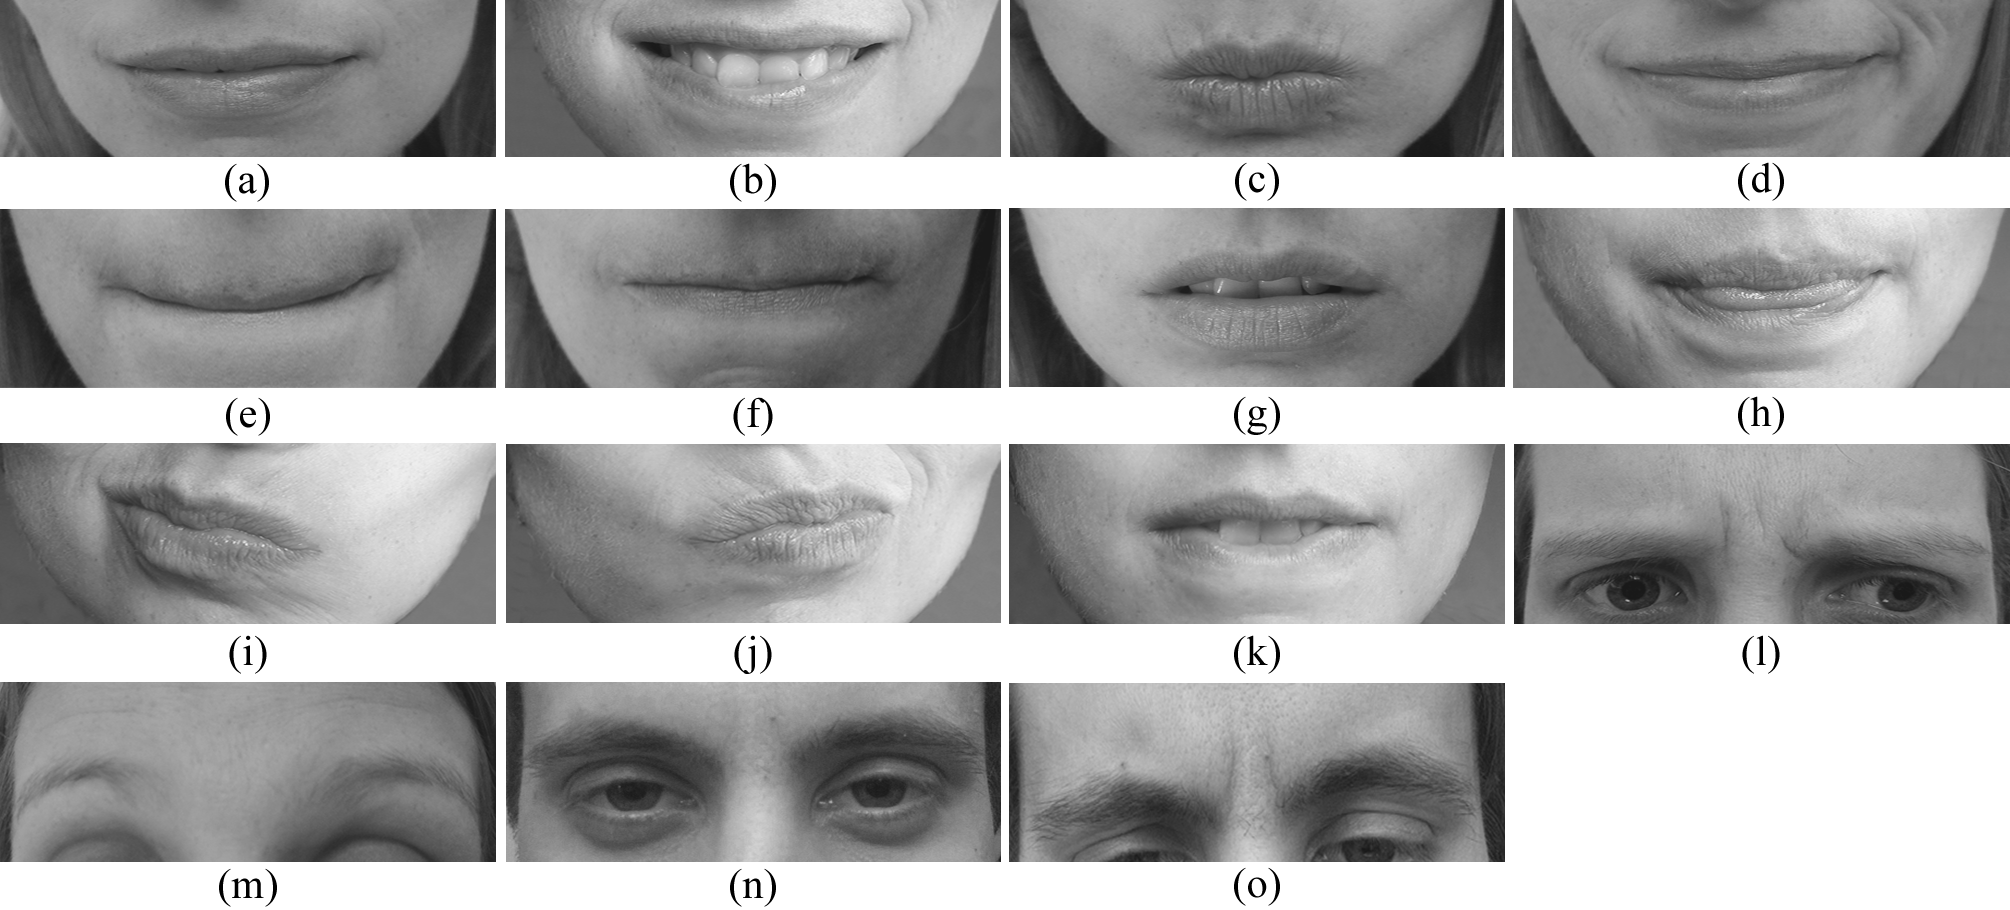
\includegraphics[width=0.4\textwidth]{Content/figures/facial-actions}
\caption{Annotated facial actions (FA). (a) Smile not showing teeth; (b) Smile showing teeth; (c) Lip puckerer; (d) Lip stretcher; (e) Lip suck; (f) Lip pressor; (g) Lips parted; (h) Tongue touching lips; (i) Mouth movement right; (j) Mouth movement left; (k) Lower lip bite; (l) Frown; (m) Brow raiser; (n) Lid tightener; (o) Brow lowering}
\label{fig:fa}
\end{figure}

According to the design of the games, subjects are supposed to perceive the experience during the beginning of the games as being more boring than the one at the end, while the experience at the end should be perceived as more stressing than the one at the beginning of the games. As a result, if the game sessions of each subject is divided in half, in theory one of the two resulting parts is more likely to be perceived as more boring by the subjects, while the other is more likely to be perceived as more stressful. Using that assumption, FA annotations were divided in two groups, the ones made during the period that corresponds to the first half ($H_0$) of the games and the ones made in the second half ($H_1$). Such division of the annotation aimed to identify any pattern regarding FA happening during periods theoretically perceived as boring or stressful. After all annotations were made, an identification of uniqueness was performed and, based on that information, the repetitions of such unique actions across the games for all subjects was counted. As a result, the frequency that each FA appeared during all game sessions was obtained, as well as when they happened (in $H_0$ or $H_1$). Any FA that appeared just a single time during the whole 6 hours recording was excluded from the list, assuming that such action was noise or probably part of another action. As a result 17 unique FA that appeared in the recordings at least twice were identified. Excluding the talking and laughing FA, Figure \ref{fig:fa} illustrates all annotated FA. Finally after all annotations were counted and categorized according to the period in the game, a per-subject evaluation regarding the frequency of FA was conducted. For each subject, an inspection was performed regarding FA that appeared in $H_1$ of all three games with a higher frequency than in $H_0$, and vice versa (appeared in $H_0$ of all three games with a higher frequency than in $H_1$).

\subsection{Results}

\begin{table}[h!]
\caption{Amount of FA annotations made for all subjects during periods $H_0$ and $H_1$ of the games}
\label{table:amount-fa}
\centering
\begin{tabular}{L{.4\linewidth}C{.2\linewidth}C{.2\linewidth}}%
\toprule%
\textbf{Game} & \textbf{Period $H_0$} & \textbf{Period $H_1$} \\
\midrule
Mushroom   & 90 & 98 \\
\midrule
Platformer & 88 & 181 \\
\midrule
Tetris     & 110 & 159 \\
\bottomrule%
\end{tabular}%
\end{table}

The number of subjects that featured a particular FA was analized, alongside with the number of repetitions of such FA, for all three games. The analysis is also divided according to the period of the game. Only FA featured by two or more subjects were considered, since it produces an analysis that is connected to more frequent FA among the whole group of subjects instead of the peculiarities of a single person. Table \ref{table:amount-fa} shows the amount of FA annotations made for all subjects during the games. According to the results, the amount of FA annotations made during $H_1$ (second half) of all three games was greater than the amount of annotations made during $H_0$ (first half). The increase in annotations during $H_1$ compared to $H_0$ was 8.8\%, 105.6\% and 44.5\% higher for the Mushroom, Platformer and the Tetris game, respectively.

Regarding the FA annotated during each game, for the Mushroom game, the three most frequent FA in $H_0$ were frown (repeated 16 times among 5 subjects), talking (12 times, 3 subjects) and tongue touching lips (9 times, 3 subjects). The three most frequent FA in $H_1$ were frown (repeated 16 times among 3 subjects), talking (13 times, 5 subjects) and lips parted (13 times, 5 subjects). By comparing most frequent FA in the two periods, both frown and talking are present, however they were not featured by a significant number of participants. In fact no more than 5 subjects (25\% of the participants) featured one of those FA. It suggests that individuals present distinct facial behaviors that are not easily generalizable, even in the same context. Curiously, two particular FA presented a significant change in the amount of repetitions and subjects between the two periods: lip pressors (from 7 to 11 repetitions, 2 to 4 subjects) and lips parted (from 5 to 13 repetitions, 2 to 5 subjects). When compared to the whole group of participants, such increase is not significant (again they represent less than 25\% of the participants), but it might be the indication of a pattern for two or three subjects. As suggested by previous work, the combination of such particular changes with another physiological signal, e.g. HR, might produce an acceptable detector for boredom/stress emotional state.

For the Platformer game, the three most frequent FA for $H_0$ were frown (19 repetitions among 3 subjects), tongue touching lips (12 repetitions, 3 subjects) and smile not showing teeth (11 repetitions, 3 subjects). For $H_1$, the FA were frown (49 repetitions, 5 subjects), smile not showing teeth (21 repetitions, 7 subjects) and lips parted (17 repetitions, 5 subjects). By comparing the FA in both periods, frown was featured by more subjects (5, representing 25\%) during the stressful part of the game, however more participants (7, representing 35\%) also featured smiles not showing teeth as well. Additionally to those FA, 25\% of the participants featured talking behavior during $H_1$, externalizing game decisions.

For the Tetris game, the three most frequent FA for $H_0$ were frown (36 repetitions among 4 subjects), smile not showing teeth (14 repetitions, 4 subjects) and lip pressor (11 repetitions, 4 subjects). For $H_1$, the FA were frown (42 repetitions among 4 subjects), lip pressor (28 repetitions, 6 subjects) and smile not showing teeth (16 repetitions, 5 subjects). By comparing those results to the most frequent FA in the Mushroom game, only frown is present in both; it is important to stress that frown was featured by less than 25\% of the participants in both games, which highlights the difficulties in finding a pattern that can be applied to all subjects to identify a boring or a stressful situation, even when the most frequent FA are used. On the other hand, two FA presented a significant change from one period to another in the Tetris game: lip pressor (from 11 to 28 repetitions, 4 to 6 subjects) and talking (from 0 to 15 repetitions, 0 to 6 subjects). Both actions were featured by 30\% of the participants, which could be further investigated in the pursue of FA that can help in the identification of emotional states. Regarding the talking FA, it has been observed from the recordings that some subjects tended to externalize in words any wrong decisions they made in the game, such as how pieces were positioned, in a similar way observed during the Platformer game; in that sense, talking could be used as an indicator of activity in the game, since it is a clear facial manifestation that happened, in this case, when players were frustrated. For further FA analysis based on a group level, see \parencite{bevilacqua2016variations}.

Finally a per-subject inspection of all annotated FA was conducted according to the procedure described in Section \ref{s:experiment1-study1-methodology}. The aim was to identify, for each subjects, which FA appeared in $H_0$ (or $H_1$) of \emph{all} three games with a higher frequency than they did in $H_1$ (or $H_0$), if any. Table \ref{table:individual} shows the results of such inspection. Marked numbers represent the frequency of a FA that was present in all three games for the specified subject and period. In total 10 participants (50\%) featured at least one FA that appeared in all three games, in the same period (boring or stressful part) with a frequency equal or greater than its appearance in the counter-period. Subject 2, for instance, featured one lip pressor during $H_0$, while the total number of times the same FA appeared in $H_1$ for all three games combined was 18. It is important to highlight that subject 16 was the only one who featured a FA more frequently in $H_0$ of all three games than he/she did during $H_1$; all other subjects featured FA more frequently in $H_1$ than in $H_0$.

\begin{table}[!h]
\caption{Subject-based frequency of FA that appeared in the same period of all three games}
\label{table:individual}
\centering
\begin{threeparttable}
\begin{tabular}{cp{.4\linewidth}cc}
\toprule%
\textbf{Subject} & \textbf{FA} & \textbf{Period $H_0$} & \textbf{Period $H_1$} \\
\toprule%
2 & Lip pressor & 1 & 18\tnote{b} \\
\midrule
15 & Lip pressor & 2 & 9\tnote{b} \\
\midrule
10 & Laughing & 2 & 19\tnote{b} \\
\midrule
14 & Laughing & 3 & 9\tnote{b} \\
\midrule
12 & Smile not showing teeth & 2 & 8\tnote{b} \\
\midrule
13 & Smile not showing teeth & 0 & 6\tnote{b} \\
\midrule
18 & Smile not showing teeth & 4 & 10\tnote{b} \\
\midrule
11 & Lips parted & 1 & 10\tnote{b} \\
\midrule
17 & Lip stretcher & 0 & 8\tnote{b} \\
\midrule
16 & Talking & 7\tnote{b} & 1 \\
\bottomrule
\end{tabular}
\begin{tablenotes}
\small
\item[b]{FA was present in all three games for the specified subject and period.}
\end{tablenotes}
\end{threeparttable}
\end{table}

\subsection{Discussion}

About the FA, even though further investigation is required, calculations indicate that subjects featured a neutral face for a longer period of time during the first half ($H_0$) of all games when compared to the second half ($H_1$). Since FA annotations were made only when the subject's face featured anything different from her/his neutral face, more annotations indicate more facial activity. Additionally the results might indicate that subjects featured more FA (different from the neutral face) under stressful situations than they did under boring situations, where a neutral face/expression is probably dominant.

The games used in the experiment were designed to gradually increase the difficulty level until the subject was not able to handle it. As a consequence, it is possible to postulate that smiles and laughs during the second half could be connected to the subject's perception that the games were too difficult to continue playing properly. On the other hand, they could indicate genuine manifestations of enjoyment during the moments the subjects felt the game was properly balanced and engaging. Regarding the other FA, such as lip pressor and lips parted, further investigation is required to accurately connect or use such actions to predict/detect emotional states, however the results show a clue about how FA variations can be different on the individual level. As previously discussed, the analysis and generalization of FA on a group level is less clear than an individual approach, since FA behavior might be specific to each person. The per-subject analysis indicated that, for a portion of the participants, at least one FA was present in the three games, in the same period for the same person. Such information might be used as the starting point for further investigation regarding FA and an individual-tailored detection model for boredom/stress, for instance.

%%%%%%%%%%%%%%%%%%%%%%%%%%%%%%%%%%%%%%%%%%%%%%%%%%%%%%%%%%%%%%%%%%%%%%%%%%%%%%%%%%%%%
%\subsection{Limitations}
%%%%%%%%%%%%%%%%%%%%%%%%%%%%%%%%%%%%%%%%%%%%%%%%%%%%%%%%%%%%%%%%%%%%%%%%%%%%%%%%%%%%%

%One potential limitation of our work is the internal validity. As previously described, the experiment was based on a one-group posttest design, which does not use a control group to measure the effects of the treatment. Such design could be criticized for having low internal validity, since it is not possible to unambiguously attribute cause and effect \parencite{kirk1982experimental}. A two-group approach could be suggested as having stronger internal validity, since it contains a control group and allows a less ambiguous conclusion. In the context of our research, however, any multiple group design implies the comparison of physiological signals and emotional perceptions among different people. Given the social and cultural background of the participants, it is virtually impossible to compare two groups of people regarding stress/boredom. People have different preferences, culture and expectations, which cause maturation and history threats to internal validity \parencite{trochim2001research}. Additionally the process of comparing variations of physiological signals among different subjects is a complex task, even when subjects are similar, e.g. same age and sex. As a consequence, a subject in a control group might present a set of variations of signals and classify a game as boring, while a similar subject in another group might classify the same game as not boring at all, presenting a different set of variations of signals. In that light, our experiment relies on a one-group experimental design to increase internal validity, since subjects were compared with themselves, which removes inter-subject differences.

%Another limitation is the empirical approach used to annotate the FA, which was not based on a formal scheme and was conducted by a single person without validation by other researchers. We believe that the exploratory nature of our study regarding FA allows the use of such approach. Our aim was not to standardize FA regarding stress/boredom, but to document the perceptions of naked-eye observations of FA in a context involving games, so that it can be used to guide further steps regarding the utilization of FA in a multifactorial analysis. A frame-by-frame annotation of our video recordings using a formal scheme, such as FACS, would be a significantly laborious and time-consuming task, which is not motivated by our exploratory and empirical approach. Another limitation is the assumption used when dividing each game session in half, presuming that the middle point of the period indicates a transition from two distinct periods: $H_0$, perceived as more boring, and $H_1$, perceived as more stressing. It is not necessarily true. Even though our data indicate that subjects perceived the beginning of the games as being boring and the end as being stressful, our point of division or the periods themselves remain an assumption. There might be moments towards the end of the game, for instance, that could be perceived as more boring or joyful depending on the subject, since each participant has her/his own specific expectations and skill level regarding games. Finally the core mechanic of the Mushroom game is based on the color of the mushrooms (instead of patterns, for instance), which is not suitable for color blind subjects.

\subsection{Conclusion}

%This paper presented the description and results of an experiment aimed at exploring the variations of heart rate (HR) and facial actions (FA) during gaming sessions with induced boredom and stress. In total twenty adults of different ages and gaming experiences participated in the experiment, where they played three different games while being recorded by a video camera and monitored by a HR sensor. The games used in the experiment were carefully designed and implemented to have a difficulty level that linearly increases over time, from a boring to a stressful point. According to self-reported answers in post-games questionnaires, participants perceived the games as being boring at the beginning and stressful at the end. Such configuration gives our experiment a novel approach for the exploration of HR and FA regarding their connection to emotional states, since information can be categorized according to the induced (and theoretically known) emotional states.

Results show that more FA annotations were made during the stressful part of the games, which indicates that participants remained with a neutral face for longer periods of time during the boring part. The analysis on group level revealed that any FA pattern was related to 5 subjects (25\% of the group) at most. In the analysis conducted on the individual level, particular patterns were found for 10 subjects (50\% of the group).

%Our findings suggest that changes in the HR during gaming sessions is a promising indicator of stress, which could be incorporated into a model aimed at emotion detection. As pointed out by previous work, a user-tailored model based on several signals, e.g. HR and FA, is more likely to detect emotional states of users. In the context where the measurement of physiological signals by physical and contact-based sensors is intrusive or not desired, e.g. remote estimation of HR, information from different channels is required. One of such additional channels of information might be facial expressions, such as the FA analysis performed in this paper. For the context of our experiment, FA analysis on an individual level produced more information to connect FA and stress/boredom emotional states. We believe that this paper contributes with information regarding HR and FA in the context of games, which can be combined to create user-tailored models for emotion detection based on different data sources.

\section{Study 2: variations of heart rate}
\label{sec:experiment1-study2}

This study presents information regarding variations of HR of subjects during the experiment. The HR data related to the game session of each subject was divided in periods of 1 minute each, whose HR mean was calculated and compared to a baseline value obtained from the HR mean of the subject during rest. Based on the self-reported answers regarding stress and boredom, HR mean was analyzed at specific periods, such as the second minute of gameplay (perceived as boring) and the last minute of gameplay (perceived as stressful).

The result of this study contributes information regarding HR in the context of games. It is a key element to create user-tailored models for emotion detection based on different data sources, e.g. HR and facial actions. The following sections presents the analysis, discussion and results of the study.

\subsection{Analysis and methods}
\label{sec:study2-methodology}

Firstly the set of HR was filtered by removing all readings obtained during the experiment whose values that were equal to zero assuming they were miss-readings. After the baseline HR value for each subject ($B_s$) was calculated as:

\begin{equation} \label{eq:baseline}
B_s = \frac{1}{2}(\overline{HR}_{r1,s} + \overline{HR}_{r2,s})
\end{equation}

where $s$ indicates the subject and $\overline{HR}_{r1,s}$, $\overline{HR}_{r2,s}$ are the mean HR during the first and the second resting period (for subject $s$), respectively. $B_s$ is assumed to be the ``expected" HR of a given subject while resting. The average difference between $\overline{HR}_{r1,s}$ and $\overline{HR}_{r2,s}$ for each subject was 2.34 bpm.

The HR mean coefficient $C_s^{g,t}$ was then calculated, which is the HR mean of a subject while playing a game during a given period of 60 seconds:

\begin{equation} \label{eq:variation}
C_s^{g,t} = \frac{1}{60}\sum_{n=1}^{60} HR_{s,g}(t\cdot 60 + n)
\end{equation}

where $s$ is the subject, $g$ is the game being played ($M$ for \underline{M}ushroom, $P$ for \underline{P}latformer or $T$ for \underline{T}etris), $t$ is the period and $HR_{s,g}(k)$ is the HR measured from subject $s$, in game $g$ at the mark of $k$ seconds. Since each subject played each game for more than 60 seconds, there is more than one period for each subject for a given game. The $t$ component of $C_s^{g,t}$ specifies which of such periods the HR mean refers to. For instance, $t=0$ comprehends the period from time 0:00 until time 1:00 of a given game, $t=1$ is the period from time 1:01 until 2:00, and so on. As an example, the HR mean coefficient $C_2^{P,1}$ is the HR mean of subject $2$ while playing the Platformer game from time 1:01 to 2:00.

HR values are specific to each individual, so the relativized HR mean coefficient, $V_s^{g,t}$, was calculated by subtracting $C_s^{g,t}$ from $B_s$ as:

\begin{equation} \label{eq:variation-normalized}
V_s^{g,t} = C_s^{g,t} - B_s
\end{equation}

$V_s^{g,t}$ accounts for values that are related to changes instead of absolute HR measurements, which are significantly more suitable for comparison among different subjects, or within the same subject.

Based on previous work regarding variations of HR and emotions, the following hypothesis was stated: the HR mean during the last minute of gameplay is greater than the HR mean during the second minute of gameplay. More specifically, the true difference in means between $V^{g,n}$ (i.e. HR means when $t=n$, where $n$ is the last minute of gameplay) and $V^{g,1}$ (i.e. HR means when $t=1$, the second minute of gameplay) is greater than zero. The dependent variable is $V$ and the null hypothesis is that the true difference in means between $V^{g,n}$ and $V^{g,1}$ is less than or equal to zero. The reason why $t=1$ (second minute of gameplay) was chosen instead of $t=0$ (first minute of gameplay) for the hypothesis is because it is believed the first minute of the game might not be ideal for a fair comparison. Firstly during the first minute of gameplay, subjects are less likely to be in their usual neutral emotional state. They are more likely to be stimulated by the excitement of the initial contact with a game soon to be played, which interferes with any feelings of boredom. Secondly subjects need a basic understanding and experimentation with the game in order to judge if it is boring or not. As per the understanding of the author, such conjecture is less likely to be fulfilled during the first minute of gameplay then it is to be during the second minute of gameplay.

\subsection{Results}

Table \ref{table:hr} presents the values of $V$, the relativized HR mean coefficient, for all subjects in all games, grouped by intervals of 1 minute, calculated according to the description in Section \ref{sec:study2-methodology}. Column $g$ is the game being played, $t$ is the period in the game and $s$ is the subject. Since all games were constantly changing in difficulty and subjects have different gaming skills, there are subjects with no data entry for some $t$ intervals, which means he/she was defeated by the game earlier than other subjects were. Subject 9 had problems playing the Platformer game, so data for that subject in that game was not used in the calculations.

A positive value in Table \ref{table:hr} represents a $V$ (HR mean) that is above the subject's baseline $B_s$ (mean HR while resting) for an specific period $t$. A negative value indicates that $V$ in that period is below the subject's baseline $B_s$. Assuming $n$ as the last minute of gameplay of a given subject in a game, by comparing the values at $t=0$ (first minute of the gameplay, perceived as boring) and $t=n$ (last minute of gameplay, perceived as stressful) in the Mushroom game, 19 subjects (95\%) presented $V^{M,n}$ greater than $V^{M,0}$. The same comparison regarding the Platformer game indicates that 16 subjects (84.2\%) had higher $V^{P,n}$ than $V^{P,0}$. In the Tetris game 13 subjects (65\%) presented higher $V^{T,n}$ than $V^{T,0}$.

\begin{landscape}
\begin{table*}
\renewcommand{\arraystretch}{1.0}
\caption{Values of $V_s^{g,t}$, the relativized HR mean coefficient, for all subjects ($s$) in a given game $g$ (M is for Mushroom, P for Platformer and T for Tetris), grouped by intervals ($t$) of 1 minute}
\label{table:hr}
\centering
\begin{threeparttable}
\resizebox{1.45\textwidth}{!}{
\begin{tabular}{cccccccccccccccccccccc}
\toprule%
$g$ & $t$  & \multicolumn{20}{c}{$s$} \\
\midrule%
 & & 1    & 2    & 3    & 4    & 5     & 6    & 7    & 8    & 9    & 10   & 11    & 12    & 13   & 14   & 15    & 16   & 17   & 18   & 19   & 20 \\
\midrule%
\multirow{7}{*}{M}    & 0   & -3.8 & 2.2  & -2.5 & -3.1 & -3.4  & -2.5 & 0.4  & 3.5  & -4.9 & -2.8 & -3.4  & -0.2  & -1.8 & 5.9  & -4.9  & 6.5  & -0.4 & -3.3 & 4.4  & 2.1  \\
                      & 1   & -9.1 & -1.4 & 0.3  & -2.6 & 0.2   & -3.7 & -1.5 & 2.7  & -4.9 & -4.1 & -10.3 & 0.0   & -3.1 & -3.1 & 0.2   & 5.6  & 2.5  & -0.8 & 0.5  & 3.2  \\
                      & 2   & -4.8 & -1.3 & -0.1 & -0.6 & 7.0   & 0.9  & 2.0  & 4.5  & -0.8 & -3.0 & -9.2  & 4.1   & 0.1  & -0.5 & -0.1  & 5.4  & 2.8  & 2.4  & 2.6  & 4.8  \\
                      & 3   & -4.9 & -0.7 & -2.8 & -1.5 & 1.5   & 0.3  & 2.4  & 5.1  & -2.4 & 1.7  & -4.6  & 2.4   & 0.4  & -0.2 & 0.7   & 4.5  & 3.4  & 3.8  & 2.4  & 3.5  \\
                      & 4   & -3.9 & -1.1 & 0.9  & 1.5  & 5.3   & 0.8  & 4.5  & 6.3  & 2.0  & 1.3  & -3.6  & 3.3   & 1.6  & 6.9  & 0.0   & 4.5  & 2.9  & 3.4  & 9.9  & 9.1  \\
                      & 5   & 0.3  & 2.4  & 1.4  & 1.7  & 11.9  & -1.2 & -    & -    & 4.4  & 10.2 & 1.6   & 6.2   & -    & -    & 3.2   & -    & 5.9  & 3.2  & 17.9 & 5.8 \\
                      & 6   & -    & -    & -1.2 & -0.1 & -     & -    & -    & -    & -    & -    & -     & -     & -    & -    & -     & -    & 3.3  & -    & -    & 6.7     \\
\midrule%
\multirow{5}{*}{P}    & 0   & -1.7 & 1.3  & 0.4  & -0.2 & 0.1   & 9.9  & 2.4  & -1.7 & -\tnote{a}   & -1.9 & -2.7  & 0.8    & 5.7  & 19.7 & 6.0  & 0.2  & 5.9  & -1.2 & 4.2  & 5.5  \\
                      & 1   & -1.6 & -0.4 & 3.4  & -0.9 & -0.3  & 2.2  & 2.4  & 5.5  & -\tnote{a}   & 2.4  & -4.4  & 0.7    & -1.5 & 4.1  & 4.9  & -1.0 & 0.8  & -0.2 & 3.7  & 7.7  \\
                      & 2   & 1.9  & 9.7  & 0.8  & -0.6 & 3.0   & -1.1 & 1.3  & 3.9  & -\tnote{a}   & 15.1 & 0.2   & 3.5    & 3.9  & 3.8  & 11.7 & -0.7 & 2.8  & 0.4  & 4.0  & 10.6 \\
                      & 3   & 3.0  & 9.3  & 2.5  & -2.6 & 2.8   & 10.3 & 4.9  & 5.2  & -\tnote{a}   & 21.6 & 3.2   & 5.4    & 9.2  & 4.6  & 9.9  & -    & 2.1  & 2.6  & 7.9  & 10.4 \\
                      & 4   & 5.9  & 6.8  & -    & 8.0  & 5.3   & -    & -    & -    & -\tnote{a}   & -    & -     & -      & 4.9  & -    & 13.5 & -    & -    & -    & -    & -     \\
\hline
\multirow{6}{*}{T}    & 0   & 2.1  & 6.5  & -2.1 & -1.3 & -4.0  & 5.7  & 3.4  & 4.2  & 8.3  & 3.2  & 2.1   & -0.1  & 3.5  & 3.4  & 4.4  & -1.2 & 7.8  & -3.9 & 5.8  & 4.7  \\
                      & 1   & -2.7 & 0.0  & -3.3 & -1.2 & -4.9  & -0.1 & 4.3  & 4.2  & 2.7  & 2.9  & 0.0   & 2.6   & 2.2  & -2.5 & 5.9  & -1.3 & 4.2  & -0.4 & 5.7  & 0.0 \\
                      & 2   & -1.7 & 2.6  & 2.4  & -0.1 & -2.3  & 4.3  & 3.5  & -0.4 & 2.7  & 5.1  & 2.6   & 5.9   & 1.1  & -1.1 & 5.3  & -1.8 & 7.4  & 0.1  & 8.1  & 4.3  \\
                      & 3   & -1.9 & -0.2 & 0.3  & -2.2 & 0.8   & 5.4  & 2.1  & 3.8  & -    & 5.2  & 2.2   & 5.4   & -0.5 & -2.5 & 4.7  & -1.2 & 10.6 & 1.5  & 3.8  & 2.3  \\
                      & 4   & -0.8 & 3.0  & -    & 0.9  & -     & -    & -    & 7.8  & -    & 9.2  & 0.2   & 6.6   & -    & 3.4  & 5.6  & -1.2 & -    & 2.0  & 6.8  & 4.3  \\
                      & 5   & 1.5  & 7.4  & -    & -0.4 & -     & -    & -    & -    & -    & 12.9 & 7.4   & 4.5   & -    & 3.5  & 6.7  & -    & -    & -    & 6.9  & -    \\
\bottomrule
\end{tabular}
}
\begin{tablenotes}
\small
\item[a]{Subject 9 had problems playing the Platformer game, so data from this subject during this game was excluded.}
\end{tablenotes}
\end{threeparttable}
\end{table*}
\end{landscape}

As previously mentioned, the null hypothesis is that the true difference in means between $V$ at the last minute of gameplay ($t=n$) and at the second minute of gameplay ($t=1$) is less than or equal to zero. Table \ref{table:proof} shows the mean of the differences of a one-tailed paired t-test on the values of $V^{g,n}$, i.e. last minute of gameplay for a given game $g$, and $V^{g,1}$, i.e. second minute of gameplay for a given game $g$, for all games and subjects. Results indicate the difference is greater than zero with statistical significance for all games. For the Mushroom game, the mean of the differences between the last ($V^{M,n}$) and the second ($V^{M,1}$) minutes of gameplay is $6.11$ bpm ($p < 0.001$). For the Platformer game, the mean of the differences of $V^{P,n}$ and $V^{P,1}$ is $5.1$ bpm ($p < 0.001$). Finally, for the Tetris game, the mean of the differences of $V^{T,n}$ and $V^{T,1}$ is $3.33$ bpm ($p < 0.001$). Those numbers reject the null hypothesis, thus supporting the experimental hypothesis that the HR mean during the last minute of gameplay is greater than the HR mean during the second minute of gameplay, for all games.

\begin{table}
    \caption{Mean of the differences of $V^{g,t}$ at the periods $t=1$ (second minute of gameplay) and $t=n$ (last minute of gameplay), for all subjects in each game ($g$). Values in bpm (beats per minute). Significance was tested with a one-tailed paired t-test}
    \label{table:proof}
    \centering
  \begin{threeparttable}
     \begin{tabular}{lc}
        \toprule%
        \textbf{Game ($g$)} & \textbf{$V^{g,n}$, $V^{g,1}$} \\
        \midrule%
        Mushroom (M) & 6.11 ***  \\
        Platformer (P) & 5.10 ***  \\
        Tetris (T) & 3.33 *** \\
        \bottomrule%
     \end{tabular}
    \begin{tablenotes}
      \small
      \item[***]{$p < 0.001$}
    \end{tablenotes}
  \end{threeparttable}
\end{table}

In order to further explore the mean variation of HR at key periods other than the ones in our hypothesis, the mean of the differences involving $V^{g,0}$, $V^{g,1}$, $V^{g,n}$ and $V^{g,n-1}$ was calculated for all games and subjects. Results are shown in Table \ref{table:mean}. $V^{g,0}$ and $V^{g,1}$ are the values of $V$ for a given game $g$ during the first and the second minute of gameplay, respectively. $V^{g,n}$ and $V^{g,n-1}$ represent the values of $V$ for a given game $g$ during the last and the immediately before the last minute of gameplay, respectively. As previously mentioned, the value of $n$, the last minute of gameplay, is different for each subject since subjects might have been defeated by the game at different moments due to personal skill levels.

\begin{table}
\caption{Mean of the differences of $V^{g,t}$ at key periods, for all subjects in a given game $g$. Values in bpm (beats per minute)}
\label{table:mean}
\centering
\begin{tabular}{p{.21\linewidth}cccc}
\toprule%
\textbf{Game ($g$)} & \textbf{$V^{g,1}$,$V^{g,0}$} & \textbf{$V^{g,n}$,$V^{g,n-1}$} & \textbf{$V^{g,n}$,$V^{g,0}$} & \textbf{$V^{g,n-1}$,$V^{g,1}$} \\
\midrule%
Mushroom (M) & -0.87   & 2.39 & 5.23 & 3.71 \\
Platformer (P) & -1.31   & 2.57 & 3.78  & 2.52  \\
Tetris (T) & -1.71 & 1.22  & 1.62    & 2.10 \\
\bottomrule%
\end{tabular}
\end{table}

In the first two minutes of gameplay ($t=0$ and $t=1$), the mean of the differences between $V^{g,1}$ and $V^{g,0}$ is negative for all games. Those numbers suggest a higher HR mean during the first minute of the games ($t=0$) than during the second minute ($t=1$). At the last two minutes of gameplay ($t=n$ and $t=n-1$), the mean of the differences between $V^{g,n}$ and $V^{g,n-1}$ is positive for all games. Those numbers suggest a higher HR mean during the last minute of the game ($t=n$) compared to the penultimate minute ($t=n-1$). Finally regarding the last ($t=n$) and the first ($t=0$) minutes of gameplay, and the penultimate ($t=n-1$) and the second ($t=1$) minutes of gameplay, numbers suggest a higher HR mean during the last minute of the game ($t=n$) compared to the first minute ($t=0$). There is also a higher HR mean during the penultimate minute of gameplay ($t=n-1$) compared to the second minute ($t=1$).

\subsection{Discussion}

A number of subjects presented a higher value for $V$, the relativized HR mean coefficient, towards the end of the Mushroom and the Platformer games when compared to the same period of the Tetris game, as shown by Table \ref{table:hr}. Both the Mushroom and the Platformer game were completely new to the subjects, since they were developed exclusively for the experiment. For the self-reported 5-point Likert scale regarding familiarity with the games/genres, the mean value was 2.75 for the Mushroom, 2.8 for the Platformer and 3.35 for the Tetris game (5 being extremely familiar). Such numbers could indicate that subjects were less likely to predict what was going to happen in the Mushroom and the Platformer when compared to the Tetris game. It could explain the greater number of subjects with higher $V$ during the end (stressful) part of those two games when compared to the smaller number of subjects with higher $V$ at the end of Tetris. The later is a popular game and subjects were more familiarized with it, so they might be more likely to guess what is about to happen in the game, reducing anxiety levels. This is specially true if the subject is trained to deal with the inherent stress of the mechanic, for instance.

A significant number of subjects presented a negative value for $V$ in some periods. In total 16 subjects (80\%) in the Mushroom game, 11 (57.8\%) in the Platformer and 12 (60\%) in the Tetris game presented negative values. A negative value indicates that the subjects had a lower HR mean while playing the game at specific periods than while resting. After the experiment, some subjects reported discomfort during the resting period, mentioning that it was too long and boring. The resting period might have been stressful for some subjects, as they were required to rest while being seated without any entertainment, e.g. mobile phones. Another explanation for such negative values is that the calculation of the subject's baseline $B_s$ might be a weak approximation of the real HR mean of each subject during rest, since only two 140-seconds long resting situations for each subject were measured. It is likely, however, that the baseline calculation is still a good parameter, since the average difference between the mean HR of the two resting periods was significantly low, as explained in Section \ref{sec:study2-methodology}.

Regarding the confirmation of the hypothesis, the mean of the differences between $V$ at the last ($t=n$) and the second ($t=1)$ minutes of gameplay, presented in Table \ref{table:proof}, shows statistical significance in the difference for all games. It reinforces findings of previously mentioned works \parencite{vandeput2009heart, garde2002effects, bousefsaf2013remote, rodriguez2015vr, yamakoshi2007preliminary} which indicate that HR tends to be higher (above the subject's baseline) during stressful moments and lower (closer to subject's baseline) during boring moments in a gaming context. As previously described, the reason why the $t=1$ (second minute of gameplay) was used instead of $t=0$ (first minute of gameplay) for the main comparison is because the first minute of all games might not be ideal for a fair comparison. During the first minute, subject are less likely to be in their usual neutral emotional state. Such line of reasoning is supported by the exploratory analysis of the mean of the differences of $V$ at periods other than the ones used in the hypothesis, as presented in Table \ref{table:mean}. In the beginning of the games, the HR mean during $t=0$ (0:00 to 1:00) was higher than during $t=1$ (1:01 to 2:00) for all three games. It could indicate that subjects were more stimulated at the very beginning, probably caused by the excitement of the initial contact with a game to be played. Such difference during $t=1$ and $t=0$ could also be explained as a response to the fact that subjects probably understood the game mechanic. During the first minute of gameplay, subject are probably still working to understand the game, so an opinion regarding boredom is still being formed. After the one minute mark, subject are more likely to have fully understood the game, so they could judge it was boring. Additionally, a better understanding of the mechanic combined with the fact that subjects were not allowed to change the game pace, e.g. to make it more interesting, probably increased the feeling of boredom.

%%%%%%%%%%%%%%%%%%%%%%%%%%%%%%%%%%%%%%%%%%%%%%%%%%%%%%%%%%%%%%%%%%%%%%%%%%%%%%%%%%%%%
%\subsection{Limitations}
%%%%%%%%%%%%%%%%%%%%%%%%%%%%%%%%%%%%%%%%%%%%%%%%%%%%%%%%%%%%%%%%%%%%%%%%%%%%%%%%%%%%%

%One potential limitation of our work is the internal validity. As previously described, the experiment was based on a one-group posttest design, which does not use a control group to measure the effects of the treatment. Such design could be criticized for having low internal validity, since it is not possible to unambiguously attribute cause and effect \parencite{kirk1982experimental}. A two-group approach could be suggested as having stronger internal validity, since it contains a control group and allows a less ambiguous conclusion. In the context of our research, however, any multiple group design implies the comparison of physiological signals and emotional perceptions among different people. Given the social and cultural background of the participants, it is virtually impossible to compare two groups of people regarding stress/boredom. People have different preferences, culture and expectations, which cause maturation and history threats to internal validity \parencite{trochim2001research}. Additionally the process of comparing variations of physiological signals among different subjects is a complex task, even when subjects are similar, e.g. same age and sex. As a consequence, a subject in a control group might present a set of variations of signals and classify a game as boring, while a similar subject in another group might classify the same game as not boring at all, presenting a different set of variations of signals. In that light, our experiment relies on a one-group experimental design to increase internal validity, since subjects were compared with themselves, which removes inter-subject differences.

\subsection{Conclusion}

Results indicate that the average HR mean for all subjects during the last minute of gameplay was greater than the average HR mean during the second minute of gameplay, for all games with statistical significance ($p<0.001$). The findings are aligned with and reinforce previous research that indicate higher HR mean during stressful situations in a gaming context. The design of the games permitted a more elaborated analysis of boring and stressful periods, which contributes information regarding variations of HR mean during such conditions in gaming sessions. Additionally an exploratory investigation regarding HR mean during other key periods in the games was performed, e.g. first and penultimate minutes of gameplay. Further analysis is still required, however the numbers suggest that the average HR mean during the first minute of gameplay was greater than during the second minute of gameplay, probably as a consequence of unusual excitement during the first minute, e.g. the idea of playing a new game.

The findings suggest that changes in the HR during gaming sessions is a promising indicator of stress, which could be incorporated into a model aimed at emotion detection. As pointed out by previous work, a user-tailored model based on several signals, e.g. HR and FA, is more likely to detect emotional states of users.

\section{Study 3: heart rate and accuracy of rPPG measurements}
\label{s:experiment1-study3}

This study presents information regarding the accuracy evaluation of a remote photoplethysmography (rPPG) technique in a gaming context. The technique was applied to estimate the HR of subjects behaving naturally in gaming sessions with induced boredom and stress. Previous work with experiments involving emotions and rPPG were performed under extremely controlled situations with few game-related stimuli. Subjects were not interacting with a complete digital game in any of the experiments, which hindered the accuracy evaluation of rPPG techniques within the context of games research, for instance. Authors commonly used images, videos or text as content to produce the emotional stimuli, in experimental sessions lasting from 20 seconds to 10 minutes.

The aforementioned non-game stimuli content is less likely to produce the reactions of a real gaming session, e.g. spontaneous body movement and facial actions. As opposed to such works, in this study each subject spent an average of 25 minutes in the session, playing three different games that were custom-made to provoke the emotional reactions similar to a natural play session. Subjects were also not instructed regarding how they should move, so body and facial reactions are likely to be the ones the subject would normally perform under a gaming context.

The recordings of game sessions of each subject were divided in video segments of 1 minute each. The rPPG technique by Poh et al. \parencite{poh2011advancements} was applied to each of those video segments to estimate the HR of subjects. An accuracy evaluation of the estimated HR obtained from the video segments was performed in relation to the HR calculated from ground truth.

%In that context, we designed and carried out an experiment focused on the accuracy evaluation of an rPPG technique applied to real gaming sessions, using custom made games as emotion stimuli.  We aim to explore the accuracy of rPPG-estimated HR readings of subjects while playing under such circumstances. To the best of our knowledge, this is the first experiment to measure the accuracy of an rPPG technique with the use of three boredom/stress-inducing games with subjects behaving naturally.

\subsection{Analysis and methods}

Firstly the videos of each game session were divided into several video segments of 60 seconds each, denoted as $V_i$, where $i \in [1, 2, ..., n]$ represents the interval (1 comprehends the time from 0:00 until 1:00, 2 comprehends the time from 1:00 until 2:00, and so on). The use of 60 seconds as the duration of each video segment is based on the work by \textcite{poh2011advancements}.

Since the games have a constantly increasing difficulty level, different subjects might have played the same game for longer or shorter periods of time. As a consequence, the interval $n$ represents the last available interval for each subject and it is likely to be different among subjects. Any remaining video segment of less than 60 seconds was discarded, i.e. if the duration of a game session was not multiple of 60. Following was the calculation of $HR_{gt}(V_i)$, which is the mean HR obtained from the ground truth data of a subject while playing during the video segment $V_i$. It was excluded from the calculation any HR value equal to zero assuming it was a miss-reading.

As previously mentioned in Section \ref{s:literature-rppg-techniques}, the rPPG technique proposed by \textcite{poh2011advancements} is consolidated, extensively mentioned in the literature and presents the best SNR for HR estimation under non-exercising situations. For those reasons, such technique  (refereed as the rPPG technique from now on) was selected to perform the extraction of HR from the video segments. For the comparison, $HR_{video}(V_i)$ was calculated, which is the estimated HR from video segment $V_i$ obtained with the rPPG technique. The evaluation of the accuracy of $HR_{video}$ when compared to $HR_{gt}$ was based on statistical methods used by previous works \parencite{poh2011advancements, rouast2016remote, li2014remote}. The measurement error is calculated as:

\begin{equation}
\label{eqn:hr-error}
HR_{error} = HR_{video} - HR_{gt}
\end{equation}

where $HR_{video}$ is the set of HR estimations by the rPPG technique from the video segments and $HR_{gr}$ is the set of HR means calculated from the ground truth obtained from the watch, as previously described in Section \ref{s:experiment1-study3}. $HR_{error}$ was calculated with video segments of a given game (for the analysis of that game) or with all available segments (for the analysis of all games combined).

The following measurements were also calculated: mean of $HR_{error}$ denoted as $M_e$; standard deviation of $HR_{error}$ denoted as $SD_e$; root mean squared error (RMSE) of $HR_{error}$; mean of error-rate percentage, calculated as:

\begin{equation}
\label{eqn:merate}
M_{eRate} = \frac{1}{N} \sum_{i=1}^{N}\frac{|HR_{error}(V_i)|}{HR_{gt}(V_i)}
\end{equation}

where $V_i$ is a video segment and $N$ is the total of video segments for a given game (or for all games); finally the linear correlation between $HR_{video}$ and $HR_{gt}$ accessed using Pearson's correlation coefficient $r$.

%%%%%%%

The selected rPPG technique was implemented in Matlab R2016a according to the original paper by \textcite{poh2011advancements}. Since the custom algorithm to detect peaks mentioned in the article is unknown, such step was replaced by the identification of the highest peak in the frequency domain after an FFT operation. This operation is commonly used in the HR estimation phase of rPPG techniques, as explained in Section \ref{s:literature-rppg-structure}.

The implementation of the rPPG technique was validated with a procedure similar to the one described by \textcite{li2014remote}. Firstly a manual inspection of all video recordings from the experiment was performed and a segment $V'_i$ of 30 seconds (1500 frames) was exerted from each video where the subject presented the least amount of body motion and facial activity. It resulted in a testing set of 20 video segments of 30 seconds each, totalizing 30000 frames of data. The mean HR calculated from ground truth for the testing set was 76.8 bpm (SD 13.4 bpm, min. 55 bpm, max. 110 bpm).

The rPPG technique was then applied to each of those $V'_i$ segments to estimate the HR, evaluating the estimated values using ground truth and the statistical methods previously described. Results are presented in Table \ref{table:rppg-validation}. The numbers indicate the implemented rPGG technique produces accurate and statistically significant results for the estimations, which are aligned with those reported in the original paper. Therefore it is assumed the rPPG technique is correctly implemented and further accuracy measurements obtained during the analysis are due to subject activity, not implementation errors.

\begin{table}
\caption{Performance of the rPPG technique applied to the testing set}
\label{table:rppg-validation}
\centering
\begin{threeparttable}
  \begin{tabular}{ccccc}
  \toprule
    $M_e$ (bpm) & $SD_e$ (bpm) & RMSE (bpm) & $M_{eRate}$ (\%) & $r$ \\
  \midrule
    -0.25 & 1.41 & 1.40 & 1.52 & 0.99* \\
  \bottomrule
  \end{tabular}
  \begin{tablenotes}
    \small
    \item[*]{$p < 0.001$}
  \end{tablenotes}
\end{threeparttable}
\end{table}

\subsection{Results}

The performance of the rPPG technique regarding the extraction of the HR is presented on Table \ref{table:rppg-validation-games}. The first three rows of the table present the performance evaluation calculated with data from each game, while the last row presents the same performance evaluation calculated with data from all games combined. Regarding the analysis of all games combined, the mean estimation error $M_e$ was 2.99 bpm ($SD_e$ 18.83 bpm), RMSE was 19.03 bpm and $M_{eRate}$ was 10.31\%. The low value for $M_e$ suggests feasible overall accuracy of the technique, however the high values for $SD_e$ and $M_{eRate}$ suggest significant variation among the estimations.

As demonstrated by $M_{eRate}$, which is the mean of error-rate percentage, the estimation error of the rPPG technique was equivalent to 10.31\% of the expected HR value calculated from ground truth, on average. On a game level, the mean estimation error $M_e$ was 2.96 bpm ($SD_e$ 19.45 bpm) in the Mushroom game, 0.31 bpm (13.51 bpm) in the Platformer game and 5.18 bpm (21.45 bpm) in the Tetris game. RMSE and $M_{eRate}$ were 19.59 bpm and 10.88\% in the Mushroom game, 13.43 bpm and 7.82\% in the Platformer game, and 21.97 bpm and 11.64\% in the Tetris game, respectively.

All three games presented acceptable values for $M_e$ and significantly higher values for $SD_e$ and $M_{eRate}$, which also suggests feasible results with considerable variations in the estimation error during the analysis of subjects for each game. In particular, the estimations performed during the Platformer game presented the lowest values for $M_e$, RMSE and $M_{eRate}$, which indicates the rPPG technique performed with lower errors and fewer variations among subjects in the Platformer game than it did in the other two games.

\begin{table}
\caption{Accuracy measurements of the rPPG technique when applied to the video segments of a given game and of all games}
\label{table:rppg-validation-games}
\begin{threeparttable}
  \begin{tabular}{p{0.13\linewidth}ccccp{0.04\linewidth}}%
  \toprule
     Game & $M_e$ (bpm) & $SD_e$ (bpm) & RMSE (bpm) & $M_{eRate}$ (\%) & $r$ \\
  \midrule
      Mushroom & 2.96 & 19.45 & 19.59 & 10.88 & 0.45* \\
      Platformer & 0.31 & 13.51 & 13.43 & 7.82 & 0.55* \\
      Tetris & 5.18 & 21.45 & 21.97 & 11.64 & 0.37* \\
      \textit{All} & 2.99 & 18.83 & 19.03 & 10.31 & 0.43* \\
  \bottomrule
  \end{tabular}
  \begin{tablenotes}
    \small
    \item[*]{$p < 0.001$}
  \end{tablenotes}
\end{threeparttable}
\end{table}

The Pearson's correlation coefficient $r$ regarding $HR_{gt}$ (mean HR calculated from the ground truth) and $HR_{video}$ (mean HR estimated via rPPG) is 0.45, 0.55 and 0.37 for the Mushroom, Platformer and Tetris game, respectively. All correlations have statistical significance, $p < 0.001$. The correlation is illustrated in Figure \ref{fig:chart-r-games}. For all three games, there is a positive and medium strength correlation between $HR_{gt}$ and $HR_{video}$, which also indicates the estimations performed by the rPPG technique are feasible. The correlation is stronger in the Platformer game, followed by the Mushroom game and finally by the Tetris game.

\begin{figure}[!h]
\centering
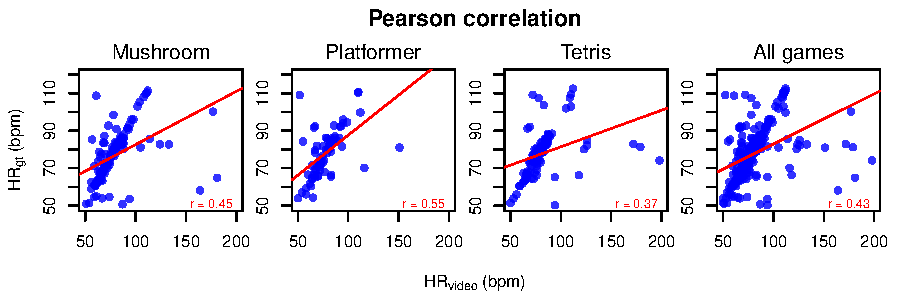
\includegraphics[width=\columnwidth]{Content/figures/correlation-hrgt-hrvideo.pdf}
\caption{Statistical correlation of $HR_{gt}$ and $HR_{video}$ when applied to the video segments of each game, as well as to the video segments of all games.}
\label{fig:chart-r-games}
\end{figure}

To better analyze the variations regarding estimation errors among subjects, figures \ref{fig:chart-hists-me} and \ref{fig:chart-hists} show a distribution of values of $M_e$, RMSE and $M_{eRate}$ for all games combined and individually. The x-axis represents intervals of values of $M_e$, RMSE or $M_{eRate}$ while the y-axis represents the percentage of subjects that presented an estimation error within the interval informed in the x-axis.

Regarding the distribution of values of $M_e$, shown in Figure \ref{fig:chart-hists-me}, overall 66.1\% of the subjects presented estimations with $M_e$ within the interval [-5 bpm, 5 bpm]. For the remaining 33.9\% of the subjects, $M_e$ was spread within the interval [-20 bpm, 35 bpm]. On a game level, $M_e$ was within the interval [-5 bpm, 5 bpm] for 65\%, 68.4\% and 65\% of the subjects of the Mushroom, Platformer and Tetris game, respectively. The values for $M_e$ are more equally distributed for the Platformer game, which explains the lower values of $SD_e$ for that game when compared to the Mushroom and the Tetris game, which present less equally distributed values of $M_e$.

The distribution of values of RMSE, shown in Figure \ref{fig:chart-hists} in the first row, indicate that overall values were lower then 10 bpm for 59.4\% of the subjects, while the remaining of the subjects had RMSE varying from 10 bpm to 50 bpm. On a game level, RMSE was lower than 10 bpm for 50\%, 68.5\% and 60\% of the subjects of the Mushroom, Platformer and Tetris game, respectively.

Regarding $M_{eRate}$, shown in Figure \ref{fig:chart-hists} in the second row, overall 69.5\% of subjects had HR estimations that were up to 10\% different than the expected HR from ground truth. On a game level, in total 73.7\% and 70\% of the estimations performed by the rPPG technique during the Platformer and the Tetris game, respectively, presented $M_{eRate}$ interior or equal to 10\%. Those values are slightly better than the 65\% of the subjects with $M_{eRate}$ up to 10\% in the Mushroom game. Despite the fact that $M_{eRate}$ was similar for both the Platformer and Tetris games, the former presented no subjects whose $M_{eRate}$ was greater than 30\%, while the later presented 10\% of the subjects with $M_{eRate}$ greater than 30\%.

\begin{figure}[!h]
\centering
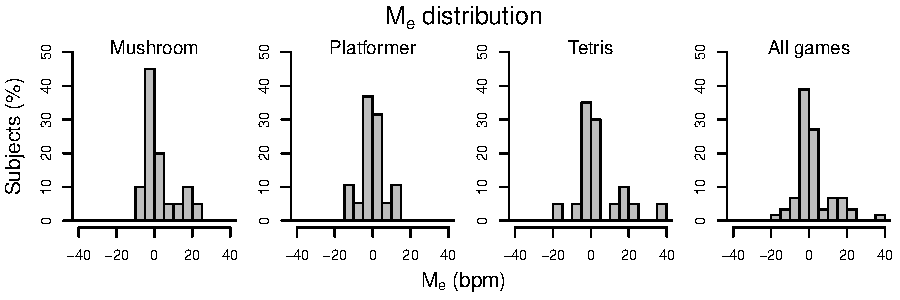
\includegraphics[width=1.0\textwidth]{Content/figures/hist-me.pdf}
\caption{Distribution of values of $M_e$ for all games. The x-axis represents intervals of values of $M_e$ while the y-axis represents the percentage of subjects that presented an estimation error within the interval informed in the x-axis.}
\label{fig:chart-hists-me}
\end{figure}

\begin{figure}[!h]
\centering
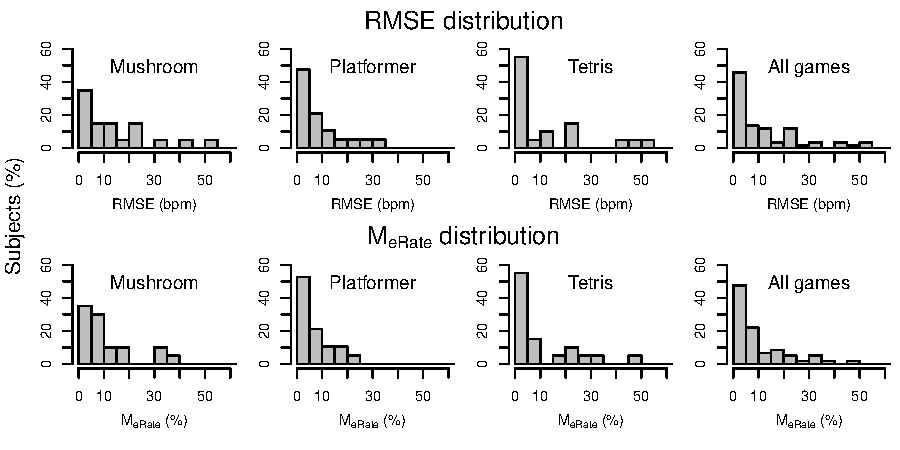
\includegraphics[width=1.0\textwidth]{Content/figures/hist-rmse-mrate.pdf}
\caption{Distribution of values of RMSE and $M_{eRate}$ for all games. The x-axis represents intervals of values of RMSE or $M_{eRate}$ while the y-axis represents the percentage of subjects that presented an estimation error within the interval informed in the x-axis.}
\label{fig:chart-hists}
\end{figure}

\subsection{Discussion}

The results obtained indicate that the use of the selected rPPG technique to estimate HR from videos of gaming sessions is feasible. When the technique was applied to a testing set of 20 manually selected 30 seconds long video segments, whose subject's facial activity and body movement were minimal, the estimations were significantly accurate. As demonstrated by Table \ref{table:rppg-validation}, the mean of error-rate $M_{eRate}$ was 1.52\% and the Pearson's correlation coefficient was $r = 0.99$ for that testing set. Those results were expected since the videos featured an unrealistic condition where subjects remained mostly still with a neutral face.

When the rPPG technique was applied to all gaming sessions, however, body movement and facial activity significantly impacted the estimation performance. It is aligned with previously described works in the literature, which indicate the estimation error increases when subject activities increase \parencite{Wang_2016novel}.

The elevated values for $SD_e$, the standard deviation of $M_e$, suggest significant variations in the estimations among subjects in each video segment. The estimation discrepancies do not seem to be caused by errors equally spread among all gaming sessions, but due to a subset of problematic ones instead. The discrepancies and skewness of the estimations are visible in the scatter plot of the estimated and expected HR values in Figure \ref{fig:chart-r-games}. It shows a cluster of points for each game, however it is surrounded by significantly wrong estimation points. In the Mushroom game, for instance, 5 estimations (bottom right of the chart) were in the interval [120 bpm, 181 bpm] bpm, which is significantly outside the expected ground truth interval of [80 bpm, 110 bpm]. Similar significantly wrong estimations can also be seen in the Platformer and the Tetris game.

The skewed distribution of values of $M_e$, $M_{eRate}$ and RMSE illustrated in figures \ref{fig:chart-hists-me} and \ref{fig:chart-hists} also support that indication. Considering the estimations for all games, in total 69.5\% of them presented $M_{eRate}$ related to an estimation value that was less than 10\% different than the expected HR from ground truth. Additionally 59.4\% of all estimations presented RMSE lower than 10 bpm. That result is slightly worse when compared to similar works that used rPPG techniques and subjects featuring natural movements, whose reported RMSE was between 0.11 and 7.28 bpm.

A direct comparison of the results of this study to the ones of such similar works is unfair however. Despite the fact that the aforementioned works present experiments where subjects are told to behave naturally, their accuracy evaluation is based on artificial human-computer interactions, as previously described in Section \ref{s:experiment1-study3}. The accuracy results of the present study account for body and facial movement caused by games whose focus is entertainment, not artificial interactions. As a consequence, the results are more connected to a scenario involving real and spontaneous reactions to games, showing that the estimations of the rPPG technique are feasible, however skewed by other factors such as natural facial activity and subject movement.

The differences in estimation also seem to be connected to the particularities of each game and subject. Considering the distribution of values of RMSE and $M_{eRate}$, both the Platformer and the Tetris games presented more estimations with lower error than the Mushroom game. The Mushroom game presented 15\% of its estimations with RMSE greater than 30 bpm and $M_{eRate}$ greater than 30\%, which are significantly wrong estimations.

In order to further explore such differences in estimations, the variations of movement and size of the ROI used to track the subject's face along the videos was analyzed. A stable ROI (both in shape and movement) is required for a precise extraction of the plethysmographic signal, so significant variations in the ROI lead to estimation errors. The mean position of the center point of the ROI for each subject in each gaming session was calculated. For each subject in each game session, the Euclidean distance between the center point of the ROI of each frame and the mean center point of the ROI previously calculated (for that subject in that session) was measured.

Similarly the mean length of the ROI diagonal for each subject in each game session was calculated, subtracting it from the length of the ROI diagonal of each frame in that gaming session. Since game sessions differ in time duration, the subject's progress in the game was normalized using the interval [0, 1], where 0 is the start point of the gaming session and 1 its end. Measurements were also subtracted from the sessions mean to facilitate analysis and comparison among different games/subjects.

\begin{figure}[!h]
\centering
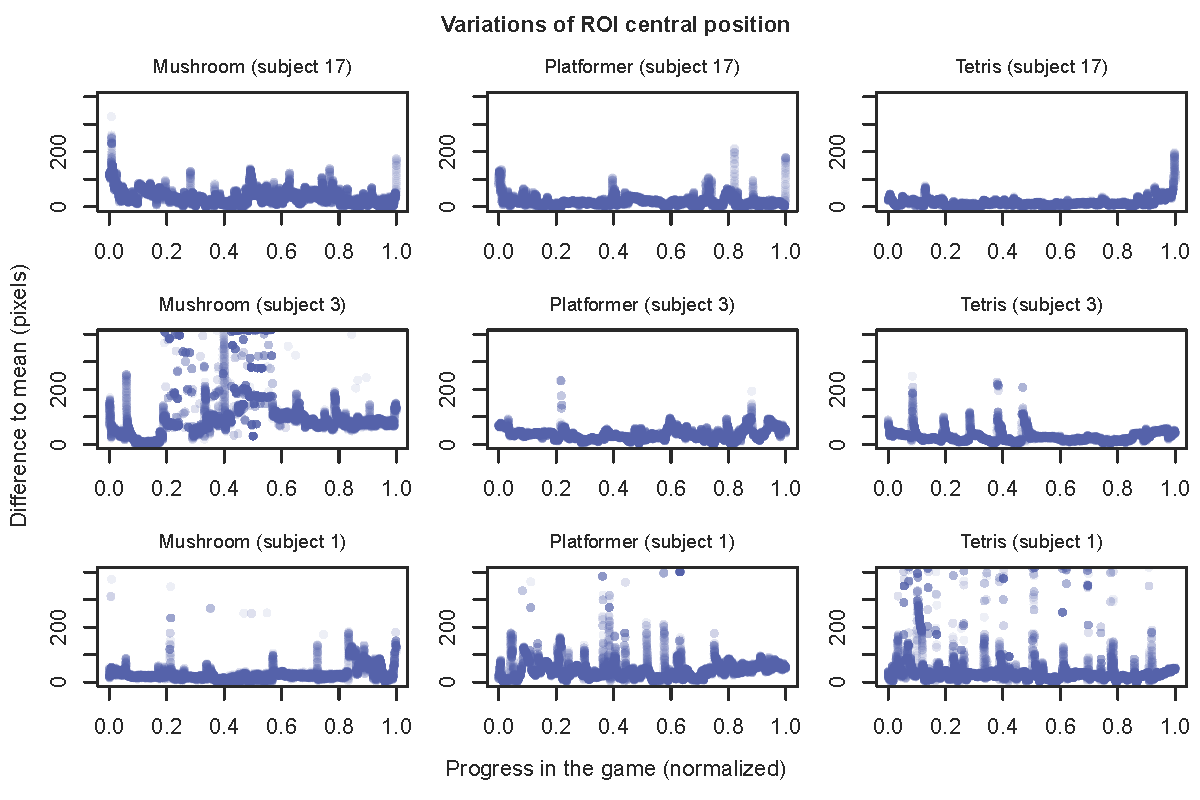
\includegraphics[width=\textwidth]{Content/figures/variation-roi-center.png}
\caption{Variations of distance of the ROI central position for subjects 17 (low estimation errors), 3 (moderate to high estimation errors) and 1 (high estimation errors) during their gaming sessions. Values were subtracted from session mean to facilitate analysis and comparison among different games/subjects.}
\label{fig:chart-roi-anomalies-center}
\end{figure}

Figure \ref{fig:chart-roi-anomalies-center} illustrates some of the patterns observed in the investigation of the distance of the ROI central position. Each row in the figure contains three charts showing the variations of the ROI central position along the gaming sessions of a given subject. The first row contains the investigation of subject 17, who presented, for all his/her gaming sessions combined, -0.33 for $M_e$ ($SD_e$ 1.4) and 1.39 for RMSE (low estimation errors). The second row shows subject 3, who presented 11.47 for $M_e$ ($SD_e$ 16.47) and 19.62 for RMSE (moderate to high estimation errors). Finally the third row shows subject 1, who presented 15.94 for $M_e$ ($SD_e$ 28.5) and 31.96 for RMSE (high estimation errors).

The estimations performed on subject 17 were significantly accurate and the charts regarding the variation of the ROI central position show a stable progression along all gaming sessions. The distance variation (y-axis) remains mostly concentrated within the interval of [0, 100] pixels for all games, which suggest the subject presented few or short movements during gaming sessions. Subject 3 also presented low variation in the Platformer and the Tetris game, however there is a significant variation in the ROI central position in the Mushroom gaming session. The chart indicates significant distance variations of the ROI that are above 200 pixels in a certain period of the game. Finally subject 1 presents high variations in the ROI distance in all gaming sessions, as demonstrated by points above the 200 pixels mark regarding the difference to mean. The Tetris game, in special, present distance variations above 200 pixels during almost the whole session.

\begin{figure}[!h]
\centering
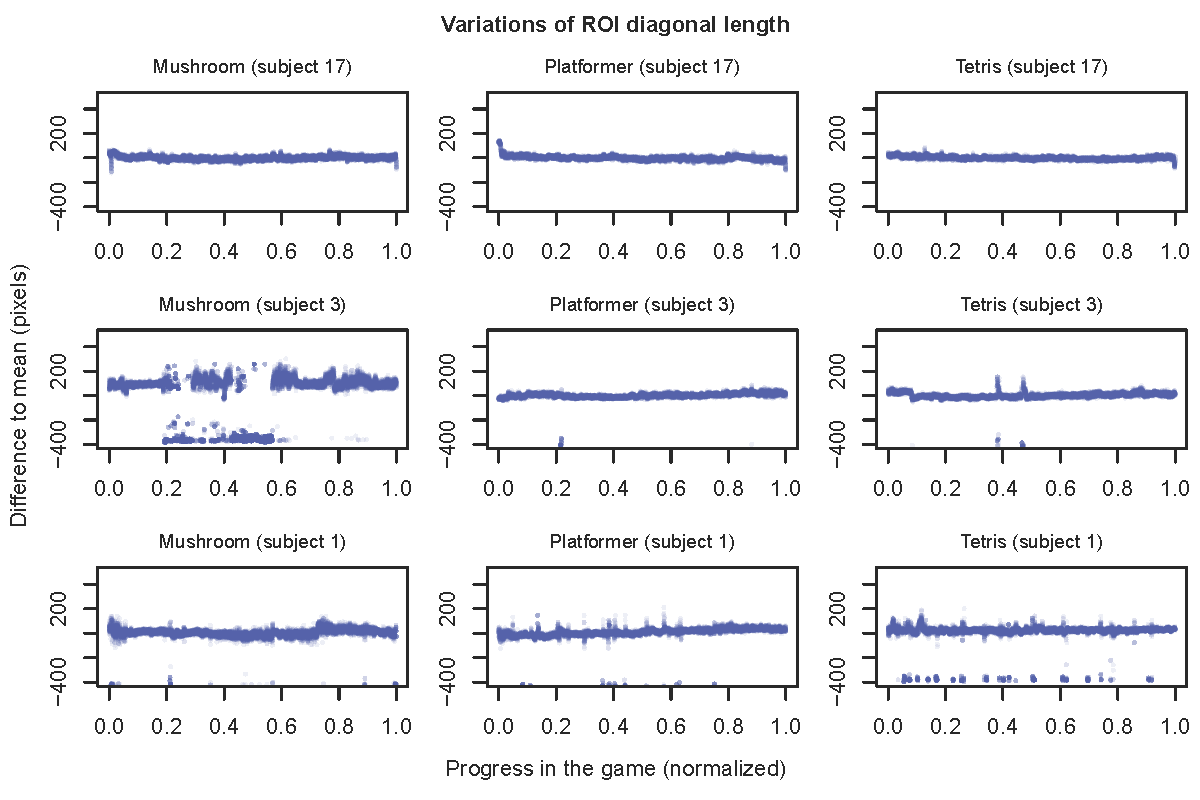
\includegraphics[width=\textwidth]{Content/figures/variation-roi-diagonal.png}
\caption{Variations of ROI diagonal length for subjects 17 (low estimation errors), 3 (moderate to high estimation errors) and 1 (high estimation errors) during their gaming sessions. Values were subtracted from session mean to facilitate analysis and comparison among different games/subjects.}
\label{fig:chart-roi-anomalies-diagonal}
\end{figure}

Figure \ref{fig:chart-roi-anomalies-diagonal} illustrates the same subjects regarding the investigation of the variations of the ROI diagonal length. Similarly to the variations of the ROI central position, the variation of the ROI diagonal length (y-axis) is lower for subject 17 (first row of charts in the figure), since the majority of the values are close to zero. Subject 3 also presents low variations in the ROI diagonal length during the Platformer and the Tetris game, however there are significant changes in the ROI size during a period in the Mushroom game. In such period, the length of the ROI diagonal is negative, i.e. -400 pixels, which indicates the size of the detected ROIs for those frames was smaller than the mean ROI diagonal length. It could be caused by a wrongly detected face (false-negative), for instance. Finally subject 1 presents, to some extent, variations of the ROI diagonal length during the majority of his/her gaming sessions. Those constant variations could be caused by the inability of the face tracking algorithm to stably and continuously detect the subjects face along the frames of the video. The chart shows a distribution of values along the zero mark regarding difference to mean, however they are more spread than those of subject 17, for instance, which indicates higher instability of the ROI size/detection for subject 1. In the Tetris session of subject 1, for instance, there are extreme variation in the ROI diagonal length with values close to -400 pixels, similarly to the ones of subject 3 in the Mushroom game. Such extreme variation could also be explained by a wrongly detected face area during those frames.

An inspection of the videos of subjects with patterns similar to the ones of subjects 3 and 1 revealed sensitive amount of movement and facial activity, including occlusion of the face by the subject's hand, as illustrated by Figure \ref{fig:face-variation}. Any facial occlusion influences the face tracking algorithm used (Viola\&Jones), since it might wrongly detect the face position or do not detect it at all. A flawed face detection step affects the extraction of the plethysmographic signal, because noise is extracted along with the raw signal, making the rPPG technique unable to separate it properly.

Despite the efforts to create games that prevented face occlusion by the subject's hand, such behavior seems to be natural in boring situations. Both Mushroom and Tetris games were more likely to allow players to place a hand in the face to express boredom, since the games could still be played with a single hand when the gameplay speed was not elevated. The Platformer game, on the other hand, is less likely to allow players to use only a single hand to play, which reduced chances of face oclusion inferering with the face tracking algorithm. This could also explain why estimations made during the Platformer game were more accurate than those performed during the other two games. Those extreme cases with facial occlusion are probably affecting the error rates in the analysis, producing less accurate estimations. Such extreme and flawed cases could have removed from the analysis, however the aim is to test how the selected rPPG technique performs in natural gaming situations. A dataset with untreated videos of gaming sessions with natural interactions might produce sub-optimal HR estimations, however it is the understanding that stressing the rPPG technique with less artificial videos provides researchers with insights about possible problems and accuracy limits of such tool.

\begin{figure}
\centering
  \begin{subfigure}[b]{0.5\textwidth}
    
\includegraphics[width=0.95\textwidth]{Content/figures/face-occlusion}
    \caption{}
    \label{fig:face-occlusion}
  \end{subfigure}%
  \begin{subfigure}[b]{0.5\textwidth}
    \centering
    
\includegraphics[width=0.95\textwidth]{Content/figures/head-tilt}
    \caption{}
    \label{fig:head-tilt}
  \end{subfigure}
  \caption{Examples of body movement and facial activity during gaming sessions. (a) Partial face occlusion by subject's hand; (b) Head tilt and movement during laugh action.}
  \label{fig:face-variation}
\end{figure}

It is possible to speculate that the variations regarding movement and size of the ROI, which directly influence estimation accuracy of the rPPG technique, seem to be connected to the unique behavior of each user as well. As illustrated by Figures \ref{fig:chart-roi-anomalies-center} and \ref{fig:chart-roi-anomalies-diagonal}, subjects present different movement patterns. Previous analysis of the videos indicates significant differences regarding facial activities among subjects \parencite{bevilacqua2016variations}. It strengthens the idea of a user-tailored model able to deal with such peculiarities, which is more likely to produce better estimations. A method that operates its estimations based on the average user behavior is prone to be significantly affected by specific user behavior outside the expected mean pattern, causing skewed distribution of estimation errors such as the ones presented on Figure \ref{fig:chart-hists} regarding $M_{eRate}$ and RMSE.

%\subsection{Limitations}

%Some limitations of the experimental procedure and analysis should be noted. The 1-minute long duration of each video segment used for the estimation of HR may affect the results. The ideal length of the video segment used for estimation (called window size) is not agreed upon in the literature \parencite{rouast2016remote}. In general, it depends on the characteristics of the rPPG technique being applied as well as the hardware configuration, such as camera framerate \parencite{roald2013estimation}. We selected a 1 min analysis window based on the information of the original work by \textcite{poh2011advancements}. Additionally our experimental procedure consists of games whose difficulty level changes every 1 minute, so that value is aligned with the window size used for HR estimation. As previously described, the statistical nature of ICA, part of the selected rPPG employed in the experiment, demands longer video samples to produce accurate results. The longer the video, however, the higher the chances of subject motion, which increases noise. A trade-off between the duration of the video segments and the estimation accuracy could be better investigated. Our experimental setup used an external light source to minimize noise caused by changes in illumination, which should narrow the estimation error to causes as subject movement and/or facial activity. It is likely, however, that other factors might impact the estimation accuracy, such as facial hair, e.g. beard and hair over the forehead area, use of glasses, and skin color.

\subsection{Conclusions}

Overall the estimation of the rPPG was feasible, showing mean estimation error of 2.99 bpm (SD 18.83 bpm), RMSE of 19.03 bpm and a positive and medium strength Pearson correlation of $r=0.43$, $p < 0.001$. On average, the estimation error of the rPPG technique was up to 10.31\% of the expected value calculated from ground truth. Additionally the exploratory investigation regarding factors that impacted the accuracy of the rPPG technique, such as variations in the region of interest (ROI) used to remotely extract the HR signal, suggest factors connected to the type of the game being played and the unique behavior of each subject influenced the estimations. Among the causes of such influence were identified body movement, e.g. head tilt and rotation, and facial occlusion by subjects hand.

\section{Study 4: automated facial analysis}
\label{sec:experiment1-study4}

This study presents a method for the automated analysis of facial cues from videos, as well as an empirical evaluation of its application as a potential tool for detecting stress and boredom in players. The proposed automated facial analysis is based on the measurement of facial features ($F_1$ to $F_7$) calculated from facial landmarks obtained unobtrusively via computer vision.

%This study introduces a method for automated analysis of facial cues from videos, presenting empirical results of its application as a potential tool for detecting stress and boredom of players in games. The method is based on Euclidean distances between automatically detected facial points, not relying on prior model training to produce results. Additionally the method is able to cope with face analysis under challenging conditions, such as when players behave naturally, e.g. moving and laughing while playing games. The method was applied on the video recordings to contextualize the automated facial analysis in a more game-oriented fashion than previous work.

%%%%%%%%%%%%%%%%%%%%%%%%%%%%%%%%%%%%%%%%%%%%%%%%%%%%%%%%%%%%%%%%%%%%%%%%%%%%%%%%%%%%%
\subsection{Facial features}
\label{sec:experiment1-study4-features-extraction}

The proposed automated facial analysis is based on the measurement of 7 facial features calculated from 68 detected facial landmarks. Table \ref{table:features} presents the facial features, which are illustrated in Figure \ref{fig:faces}(b). The facial features are mainly based on the Euclidean distances between landmarks, similar to some works previously mentioned. However, the approach does not rely on pre-defined expressions, i.e. the 6 universal facial expressions, training of a model, or the use of the MPEG-4 standard, which specifies representations for 3D facial animations, not emotional interactions in games. Additionally the method does not use an arbitrarily selected frame, e.g. the 100\textsuperscript{th} frame \parencite{giannakakis2017stress}, as a reference for calculations, since features are derived from each frame (or a small set of past frames). The features are obtained unobtrusively via computer vision analysis that focuses on detecting activity of facial muscles reported by previous work involving EMG and emotion detection in games.
%We believe our approach is more user-tailored, convenient and better suited for contexts involving games.

The process of extracting the facial features has two main steps: face detection and feature calculation. In the first step, computer vision techniques are applied to a frame of the video and facial landmarks are detected. In the second step, the detected landmarks are used to calculate several facial features related to eyes, mouth, and head movement. The following sections present a detailed description of how each step is performed, including the calculation of features.

% zygomatic -> smiling
% orbicularis oculi -> eyelid control
% corrugator -> frowning

\begin{landscape}
\begin{table*}
    \centering
    \caption{Information regarding calculated facial features}
    \label{table:features}
    \begin{tabular}[l]{@{}lcp{11cm}}
        \toprule%
            \textbf{Name} & \textbf{Notation} & \textbf{Description} \\
        \midrule%
            Mouth outer & $F_1$ & Sum of the Euclidean distance between the mouth contour landmarks and the anchor landmarks. It monitors the zygomatic muscle.  \\
            Mouth corner & $F_2$ & Sum of the Euclidean distance between the mouth corner landmarks and the anchor landmarks. It monitors the zygomatic muscle. \\
            Eye area & $F_3$ & Area of the regions bounded by the closed curves formed by the landmarks in the contour of the eyes. It monitors the orbicularis oculi muscle. \\
            Eyebrow activity & $F_4$ & Sum of the Euclidean distance between eyebrow landmarks and the anchor landmarks. It monitors the corrugator muscle.  \\
            Face area & $F_5$ & Area of the region bounded by the closed polygon formed by the most external detected landmarks.  \\
            Face motion & $F_6$ & Average value of the Euclidean norm of a set of landmarks in the last $N$ frames. It describes the total distance the head has moved in any direction in a short period of time.  \\
            Facial COM & $F_7$ & Average value of all detected landmarks. It describes the overall movement of all facial landmarks.  \\
        \bottomrule%
    \end{tabular}
\end{table*}
\end{landscape}

%%%%%%%%%%%%%%%%%%%%%%%%%%%%%%%%%%%%%%%%%%%%%%%%%%%%%%%%%%%%%%%%
\subsubsection{Face detection}

The face detection procedure is performed for every frame of the input video. Initially the face is detected using a Constrained Local Neural Field (CLNF) model \parencite{baltrusaitis2013constrained,baltruvsaitis2016openface}. CLNF uses a local neural field patch expert that learns the nonlinearities and spatial relationships between pixel values and the probability of landmark alignment. The technique also uses a non-uniform regularized landmark Mean Shift fitting technique that takes into consideration patch reliabilities. It improves the detection process under challenging conditions, e.g. extreme face pose or occlusion, which is likely to happen in game sessions (see Section \ref{sec:experiment1-study1}). The application of the CLNF model to a given video frame produces a vector $L$ of 68 facial landmarks:

\[
L = [p_0, p_1, p_2, \dots, p_{67}]^T
\]

where $p_i$ is a detected facial landmark that represents a 2D coordinate $(x_i, y_i)$ in the frame. Facial landmarks are related to different facial regions, such as eyebrows, eyes and lips. Figure \ref{fig:faces}(a) illustrates the landmarks of $L$ in a given frame.

\begin{figure}
\centering
  \begin{subfigure}[b]{0.5\textwidth}
    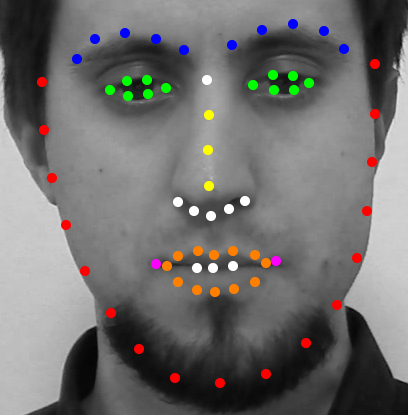
\includegraphics[width=0.95\textwidth]{Content/figures/facial-landmarks-detail.png}
    \caption{}
    \label{fig:facial-landmarks}
  \end{subfigure}%
  \begin{subfigure}[b]{0.5\textwidth}
    \centering
    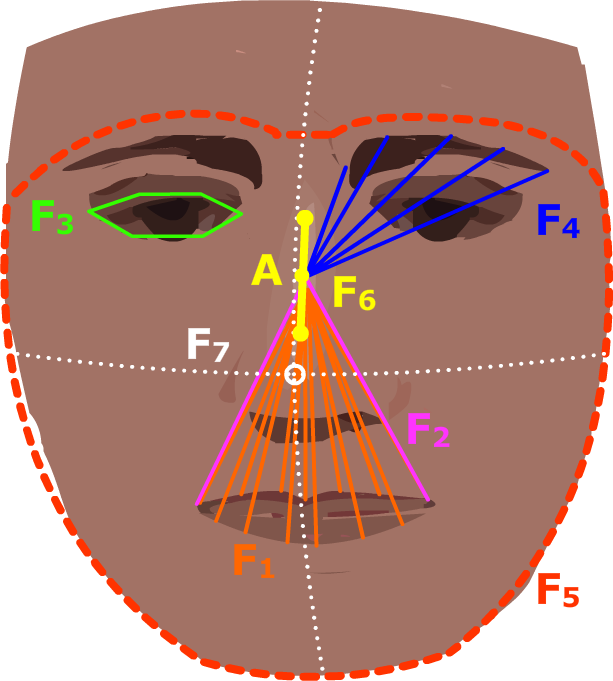
\includegraphics[width=0.95\textwidth]{Content/figures/facial-features.png}
    \caption{}
    \label{fig:facial-features}
  \end{subfigure}
  \caption{Facial landmarks and features. (a) Highlight of 68 detected facial landmarks. (b) Visual representation of the facial features.}
  \label{fig:faces}
\end{figure}


%%%%%%%%%%%%%%%%%%%%%%%%%%%%%%%%%%%%%%%%%%%%%%%%%%%%%%%%%%%%%%%%
\subsubsection{Anchor landmarks}

The calculation of the proposed facial features involves the Euclidean distance among facial landmarks. Subsequently, the Euclidean distance between two landmarks $a_1 = (x_1, y_1)$ and $a_2 = (x_2, y_2)$ is given as:

\[
d(a_1,a_2) = \sqrt{(x_2 - x_1)^2 + (y_2 - y_1)^2}
\]

Landmarks in the nose area are more likely to be stable, presenting fewer position variations in consecutive frames \parencite{giannakakis2017stress}. Consequently, they are good reference points for use in the calculation of the Euclidean distance among landmarks. In order to provide stable reference points for the calculation of our facial features, three highly stable landmarks located in the nose line were selected, denoted as the anchor vector $A = [p_{28}, p_{29}, p_{30}]^T$. The landmarks of the anchor vector $A$ are highlighted in yellow in Figure \ref{fig:faces}(a).

%%%%%%%%%%%%%%%%%%%%%%%%%%%%%%%%%%%%%%%%%%%%%%%%%%%%%%%%%%%%%%%%
\subsubsection{Feature normalization}

The subjects moved towards and away from the camera during the gaming sessions. This movement affects the Euclidean distance between landmarks, as it tends to increase when the subject is closer to the camera, for instance. Additionally, the subjects have unique facial shapes and characteristics, which also affect the calculation and comparison of the facial features between subjects. To mitigate that problem, a normalization coefficient $K$ was calculated as the Euclidean distance between the upper and lower-most anchor landmarks in $A$. In other words, $K$ represents the size of a subject's nose line. Since all features are divided by $K$, their final value is expressed as normalized pixels (relative to $K$) rather than pixels \textit{per se}.

%%%%%%%%%%%%%%%%%%%%%%%%%%%%%%%%%%%%%%%%%%%%%%%%%%%%%%%%%%%%%%%%
\subsubsection{Mouth related features}

Mouth related features aim to detect activity in the zygomatic muscles, illustrated in Figure \ref{fig:face-muscles} (c and d, page \pageref{fig:face-muscles}), which are related to changes in the mouth, such as lips activity (stretch, suck, press, parted, tongue touching, bite) and movement (including talking). Two facial features related to the mouth area were calculated: mouth outer and mouth corner.

\paragraph{Mouth outer ($F_1$):} given vector $M = [p_{48}, p_{49}, \dots, p_{60}]^T$ containing the landmarks in the outer part of the mouth (highlighted in orange in Figure \ref{fig:faces}(a)). The mouth outer feature is calculated as the sum of the Euclidean distance among the landmarks in $M$ and the anchor landmarks in $A$:

\[
F_1 = \frac{1}{K} \sum_{i=1}^{12} \sum_{j=1}^{3} d(A_j, M_i)
\]

where $A_j$ and $M_i$ are the $j$-th and $i$-th element of $A$ and $M$, respectively.

\paragraph{Mouth corner ($F_2$):} given vector $C = [p_{48}, p_{54}]^T$, containing the two landmarks representing the mouth corners (highlighted in pink in Figure \ref{fig:faces}(a)). The mouth corner feature is the sum of the Euclidean distance among the landmarks in $C$ and $A$:

\[
F_2 = \frac{1}{K} \sum_{i=1}^{2} \sum_{j=1}^{3} d(A_j, C_i)
\]

where $A_j$ and $C_i$ are the $j$-th and $i$-th element of $A$ and $C$, respectively.

%%%%%%%%%%%%%%%%%%%%%%%%%%%%%%%%%%%%%%%%%%%%%%%%%%%%%%%%%%%%%%%%
\subsubsection{Eye related features}

Eye related features aim to detect activity related to the orbicularis oculi and the corrugator muscles, illustrated in Figure \ref{fig:face-muscles}(b) and Figure \ref{fig:face-muscles}(a) respectively, which comprehend changes in the eyes region, including eye and eyebrow activity. Two facial features related to the eyes were calculated: eye area and eyebrow activity.

\paragraph{Eye area ($F_3$):} given vector $Y_l = [p_{36}, p_{37}, \dots, p_{41}]^T$ containing the landmarks describing the left eye, highlighted in green in Figure \ref{fig:faces}(a), and vector $Y_r = [p_{42}, p_{43}, \dots, p_{47}]^T$ containing the landmarks describing the right eye, highlighted in green in Figure \ref{fig:faces}(a). The eye area feature is the area of the regions bounded by the closed curves formed by the landmarks in $Y_l$ and $Y_r$, divided by $K$. The area of the curves is calculated using OpenCV's \texttt{contourArea()} function, which uses Green's theorem \parencite{stewart2011calculus}.

\paragraph{Eyebrow activity ($F_4$):} calculated as the sum of the Euclidean distances among the eyebrow landmarks and the anchor landmarks in $A$. Given the vector $W_l = [p_{17}, p_{18}, \dots, p_{21}]^T$ containing the landmarks describing the left eyebrow, highlighted in blue in Figure \ref{fig:faces}(a), and the set $W_r = [p_{22}, p_{23}, \dots, p_{26}]^T$ containing the landmarks describing the right eyebrow, highlighted in blue in Figure \ref{fig:faces}(a). The eyebrow activity feature is calculated as:

\[
F_4 = \frac{1}{K} \sum_{i=1}^{5} \sum_{j=1}^{3} \Big[ d(A_j, W_{l,i}) + d(A_j, W_{r,i}) \Big]
\]

where $A_j$, $W_{l,i}$ and $W_{r,i}$ are the $j$-th, $i$-th and $i$-th element of $A$, $W_l$ and $W_r$, respectively.

%%%%%%%%%%%%%%%%%%%%%%%%%%%%%%%%%%%%%%%%%%%%%%%%%%%%%%%%%%%%%%%%
\subsubsection{Head related features}

Head related features aim to detect body movements, in particular, variations of head pose and amount of motion the head/face performs over time. Three features related to the head were calculated: face area, face motion and facial center of mass (COM).

\paragraph{Face area ($F_5$):} during the interaction with a game, subjects tend to move towards (or away from) the screen, which causes the facial area in the video recordings to increase or decrease. Given vector $F = [p_{0}, p_{1}, \dots, p_{16}]^T$ containing the landmarks describing the contour of the face, highlighted in red in Figure \ref{fig:faces}(a). The face area feature is the area of the region bounded by the closed curves formed by the landmarks in $F \cup W_r \cup W_l$, divided by $K$. Similar to the eye area, the area under the curves is calculated using OpenCV's \texttt{contourArea()} function.

\paragraph{Face motion ($F_6$):} accounts for the total distance the head has moved in any direction in a short period of time. For each frame of the video, the currently detected anchor vector $A$ is saved, which produces vector $D = [A_1, A_2, \dots, A_n]^T$, where $A_i$ is the vector $A$ detected in the $i$-th frame of the video and $n$ is the number of frames in the video. Subsequently the face motion feature is calculated as:

\[
F_6 = \frac{1}{K} \sum_{j=1}^{3} \sum_{t=1}^{Z - 1} || D(f - t, j) - D(f - Z, j) ||
\]

where $Z$ is the number of frames to include in the motion analysis, $D(i,j)$ is the $j$-th element of $A_i \in D$, $f$ is the number of the current frame, and $||.||$ is the Euclidean norm. In the analysis presented here, a value of $Z=50$ (50 frames, equivalent to 1 second) was used.

\paragraph{Facial COM ($F_7$):} describes the overall movement of all facial landmarks. A single 2D point, calculated as the average of all landmarks in $L$, is used to monitor the movement. The COM feature is calculated as:

\[
F_7 = \frac{1}{K} \frac{1}{N} \sum_{i=1}^{N} || p_i ||
\]

where $N$ is the total number of detected landmarks (elements in $L$) and $||.||$ is the Euclidean norm.

%%%%%%%%%%%%%%%%%%%%%%%%%%%%%%%%%%%%%%%%%%%%%%%%%%%%%%%%%%%%%%%%
\subsection{Analysis and methods}
\label{sec:experiment1-study4-feature-analysis}

%%%%%%%%%%%%%%%%%%%%%%%%%%%%%%%%%%%%%%%%%%%%%%%%%%%%%%%%%%%%%%%%
\subsubsection{Data pre-processing}

The pre-processing of video recordings involved the extraction of parts containing the interaction with the games and the discarding of noisy frames. Firstly, the periods showing subjects playing each available game were extracted from the video recordings. This resulted in three videos per subject, denoted as $V_{s,i}$ where $s$ is the $s$-th subject and $i \in \{1, 2, 3\}$ represents the game.

\begin{figure}
\centering
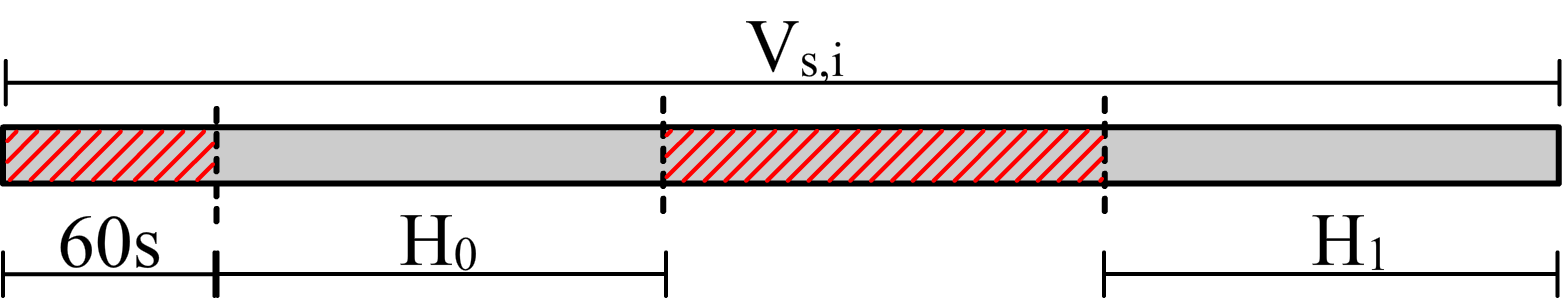
\includegraphics[width=0.7\textwidth]{Content/figures/pre-processing}
\caption{Extraction of video segments $H_0$ and $H_1$ containing boring and stressful game interactions, respectively. Initial $D$ seconds of any video $V_{s,i}$ are ignored and the remaining is divided into three pieces, from which the first and the last ones are selected. Stripes highlight discarded video segments.}
\label{fig:preprocessing}
\end{figure}

As previously mentioned, the games used as emotional elicitation material in the experiment induced variations of physiological signals in the subjects, who perceived the games boring at the beginning and stressful at the end. Since the aim of the present study was to test the potential of facial features to differentiate emotional states of boredom and stress, two video segments were extracted from each video $V_{s,i}$, named $H_0$ and $H_1$, whose subject's emotional state was assumed to be known and related to boredom and stress. In order to achieve that, the following extraction procedure was performed, illustrated in Figure \ref{fig:preprocessing}. Firstly a duration of $D$ seconds of any given video $V_{s,i}$ was ignored. For this pre-processing, $D=60$ was used. The remainder of the video was then divided into three segments, from which the first and the last were selected as $H_0$ and $H_1$, respectively.

The reason $D=60$ seconds was discarded from all the video's segments is because the initial minute might not be ideal for a fair analysis. During the first minute of gameplay, subjects are less likely to be in their usual neutral emotional state. They are more likely to be stimulated by the excitement of the initial contact with a game soon to be played, which interferes with any feelings of boredom. Additionally, subjects need basic experimentation with a game to learn how to play it and assess whether it is boring or not. This claim is supported by the empirical analysis of the first minute of the video recordings, which show repeated head and eye movements to and from the keyboard/display. Consequently, the second minute and onward in the videos is more likely to portray facial activity related to emotional reactions to the game than facial activity connected to gameplay learning. Regarding the division of the remaining part of the video into three segments, from which two were selected as $H_0$ and $H_1$, it followed the reasoning that the emotional state of the subjects was unknown in the middle part of $V_{s,i}$. Based on the self-reported emotional states, subjects reported the beginning part of the games as boring and the final part as stressful. Additionally, there are significant differences in the HR mean between the second and the last minute of gameplay in the games \parencite{bevilacqua2018changes}. As a consequence, it is assumed that the video segments $H_0$ and $H_1$ accurately portray the interaction of the subjects during boring and stressful periods of the games, respectively.

The pre-processing of the recordings resulted in 6 video segments per subjects: 3 segments $H_0$ (one per game) and 3 segments $H_1$ (one per game). A given game $i$ contains $N=20$ pairs of $H_0$ and $H_1$ video segments (20 segments $H_0$, one per subject, and 20 segments $H_1$, one per subject). With regard to all the subjects and games, there are $N=60$ pairs of $H_0$ and $H_1$ video segments (3 games $\times$ 20 subjects, resulting in 60 segments $H_0$ and 60 segments $H_1$). Subject 9 had problems playing the Platformer game, consequently, segments $H_0$ and $H_1$ from subject 9 in the Platformer game were discarded. Therefore, the Platformer game contains $N=19$ pairs of $H_0$ and $H_1$ video segments; regarding all the games and subjects, there are $N=59$ pairs of $H_0$ and $H_1$ video segments.

%%%%%%%%%%%%%%%%%%%%%%%%%%%%%%%%%%%%%%%%%%%%%%%%%%%%%%%%%%%%%%%%
\subsubsection{Feature analysis}

The previously mentioned features can be calculated for each frame of any given video, however facial cues might be better contextualized if analyzed in multiple frames. For that reason, the facial analysis was applied to all the frames of all the video segments $H_0$ and $H_1$. The mean value of each facial feature in each video segment was then calculated. As a result, any facial feature $F_i$ has $N=59$ pairs of mean values (59 from $H_0$ and 59 from $H_1$). Henceforth, the set of mean values in $H_0$ or $H_1$ of a given feature $F_i$ will be referred to simply as feature value in $H_0$ or $H_1$, respectively.
%Each mean value was calculated from all frames of a video segment ($H_0$ or $H_1$) of a subject in a particular game.

Based on a previous manual analysis of facial actions of the video recordings \parencite{bevilacqua2016variations} and findings of related work, the values of facial features during boring periods of the games are expected to be different than those during stressful periods. Since the subjects perceived the games as boring at the beginning and stressful at the end, it is assumed that values in $H_0$ and $H_1$, for all features, are likely to correlate with an emotional state of boredom and stress, respectively. Therefore, the overarching hypothesis is stated as follows: the mean value of features in $H_0$ is different than the mean value in $H_1$, for all the subjects and games. More specifically, the overarching hypothesis can be described as 7 sub-hypotheses, denoted $u_i$, where $i \in \{1, 2, ..., 7\}$. Hypothesis $u_i$ states that the true difference in means between the value of a given feature $F_i$ in $H_0$ and $H_1$, for all the subjects, is greater than zero. The dependent variable of $u_i$ is $F_i$ and the null hypothesis is that the true difference in means between $H_0$ and $H_1$ for feature $F_i$, for all the subjects and games, is equal to zero.

Hypothesis $u_i$ was tested by performing a paired two-tail t-test on the values $H_0$ and $H_1$ of feature $F_i$. In total, 7 tests were performed: $u_1$ (mouth outer), $u_2$ (mouth corner), $u_3$ (eye area), $u_4$ (eyebrow activity), $u_5$ (face area), $u_6$ (face motion), and $u_7$ (facial COM).

%%%%%%%%%%%%%%%%%%%%%%%%%%%%%%%%%%%%%%%%%%%%%%%%%%%%%%%%%%%%%%%%%%%%%%%%%%%%%%%%%%%%%
\subsection{Results}
%%%%%%%%%%%%%%%%%%%%%%%%%%%%%%%%%%%%%%%%%%%%%%%%%%%%%%%%%%%%%%%%%%%%%%%%%%%%%%%%%%%%%

Table \ref{table:changes} presents the mean of differences of all the features between periods $H_0$ and $H_1$, calculated for all the subjects in all the games, according to the description in Section \ref{sec:experiment1-study4-features-extraction}, and analyzed according to the procedures described in Section \ref{sec:experiment1-study4-feature-analysis}. The mean of differences of all the features shows a decrease from $H_0$ to $H_1$. Comparing the mean difference of a feature to its mean value in $H_0$, the decrease from $H_0$ to $H_1$ was 10.7\% for mouth outer ($F_1$), 11.8\% for mouth corner ($F_2$), 10.4\% for eye area ($F_3$), 8.1\% for eyebrow activity ($F_4$), 9.4\% for face area ($F_5$), 8.2\% for face motion ($F_6$), and 11\% for facial COM ($F_7$). Changes related to $F_6$ and $F_7$ were not statistically significant. All the remaining features presented statistically significant changes from $H_0$ to $H_1$. The greatest decrease with statistical significance was associated with mouth corner, followed by mouth outer, eye area, face area, and eyebrow activity. These numbers support the experimental expectations that values for facial features are different when a comparison is made between two distinct parts of the games, i.e. boring and stressful ones.

\begin{table}
    \caption{Mean of differences ($\pm$SD) of features between periods $H_0$ and $H_1$ ($N=59$). Units expressed in normalized pixels.}
    \label{table:changes}
    \centering
    \begin{threeparttable}
        \begin{tabular}{lc}
            \toprule%
                \textbf{Feature (notation)} &  \\
            \midrule%
                Mouth outer ($F_1$)      & -20.59 $\pm$ 57.36\textsuperscript{**} \\
                Mouth corner ($F_2$)     & -3.90 $\pm$ 10.16\textsuperscript{**} \\
                Eye area ($F_3$)         & -0.019 $\pm$ 0.064\textsuperscript{*} \\
                Eyebrow activity ($F_4$) & -15.59 $\pm$ 49.71\textsuperscript{*} \\
                Face area ($F_5$)        & -2.60 $\pm$ 7.90\textsuperscript{*} \\
                Face motion ($F_6$)      & -44.97 $\pm$ 326.74 \\
                Facial COM ($F_7$)       & -0.029 $\pm$ 0.113 \\
            \bottomrule%
        \end{tabular}
        \begin{tablenotes}
          \small
          \item[*]{$p < 0.05$}
          \item[**]{$p < 0.01$}
        \end{tablenotes}
    \end{threeparttable}
\end{table}

The two facial features related to mouth, i.e. mouth corner and mouth outer, presented a combined average decrease of 11.24\% from $H_0$ to $H_1$. The change was the most significant compared to all other features. The mean of differences of $F_1$ and $F_2$ between periods $H_0$ and $H_1$ was $T(59) = -20.59$ (SD 57.36, $p < 0.01$) and $T(59) = -3.9$ (SD 10.16, $p < 0.01$), respectively. Both features had a statistically significant change from $H_0$ to $H_1$, which supports the claim that they are different in those periods. Additionally, both features presented SD as considerably greater than the mean, which indicates that the differences of such features for each subject between periods $H_0$ and $H_1$ are likely to be spread out rather than clustered around the mean value.
Features related to eyes, i.e. eye area and eyebrow activity, presented a combined average decrease of 9.28\% from $H_0$ to $H_1$. The mean of differences of $F_3$ and $F_4$ between periods $H_0$ and $H_1$ was $T(59) = -0.019$ (SD 0.064, $p < 0.05$) and $T(59) = -15.59$ (SD 49.71, $p < 0.05)$, respectively. Similar to mouth-related features, eye-related features had a statistically significant change from $H_0$ to $H_1$, indicating that they are different in those periods. Following the same pattern of change for $F_1$ and $F_2$, both features $F_3$ and $F_4$ also presented a SD considerably greater than the mean, also suggesting that the differences of such features for each subject between periods $H_0$ and $H_1$ are likely to be spread out rather than clustered around the mean value.

Finally, features related to the whole face, i.e. face area, face motion, and facial COM, presented a combined average decrease of 9.52\% from $H_0$ to $H_1$. The mean of differences of $F_5$, $F_6$ and $F_7$ were $T(59) = -2.60$ (SD 7.90, $p < 0.05$), $T(59) = -44.97$ (SD 326.74, $p = 0.29$), and $T(59) = -0.029$ (SD 0.113, $p = 0.052$), respectively. Face area was the only feature in this category to present a change that was statistically significant between periods $H_0$ and $H_1$, supporting the idea that $F_5$ is different in those periods. In constrast, $F_6$ and $F_7$ lack statistically significant differences between periods $H_0$ and $H_1$. Similar to facial features related to mouth and eyes, features $F_5$, $F_6$ and $F_7$ presented considerably greater SD than the mean, also suggesting that the differences of such features between periods $H_0$ and $H_1$ are likely to be spread out rather than clustered around the mean value.

%%%%%%%%%%%%%%%%%%%%%%%%%%%%%%%%%%%%%%%%%%%%%%%%%%%%%%%%%%%%%%%%%%%%%%%%%%%%%%%%%%%%%
\subsection{Discussion}
%%%%%%%%%%%%%%%%%%%%%%%%%%%%%%%%%%%%%%%%%%%%%%%%%%%%%%%%%%%%%%%%%%%%%%%%%%%%%%%%%%%%%

The overarching hypothesis states that the mean value of features in $H_0$ is different than the mean value in $H_1$. Furthermore, the overarching hypothesis is composed of 7 sub-hypotheses. i.e. $u_i$, one for each feature $F_i$, where $u_i$ states that the true difference in means between the value of a given feature $F_i$ in $H_0$ and $H_1$, is greater than zero. The majority of the calculated facial features, i.e. mouth outer ($F_1$), mouth corner ($F_2$), eye area ($F_3$), eyebrow activity ($F_4$), and face area ($F_5$), presented statistically significant differences in their mean values when a comparison is made between two distinct parts of the games, i.e. $H_0$ and $H_1$. As previously mentioned, the subjects perceived the first part of the games, i.e. $H_0$, as boring and the second part, i.e. $H_1$, as stressful. The results support the claim of sub-hypotheses $u_1$ to $u_5$, which indicate that facial features $F_1$ to $F_5$ can be differentiated between periods $H_0$ and $H_1$ and can consequentially have the potential to unobtrusively differentiate the emotional states of boredom and stress of players in gaming sessions. The results refute sub-hypotheses $u_6$ and $u_7$, since features $F_6$ and $F_7$ lack statistically significant differences between periods $H_0$ and $H_1$.

Mouth related facial features, i.e. mouth outer ($F_1$) and mouth corner ($F_2$), presented statistically significant differences between boring and stressful parts of the games. Both features are calculated on the basis of the distance between mouth and nose related facial landmarks, which presented a decrease in stressful parts of the games. This decrease could be attributed to landmarks in the upper and lower lips being closer to each other, which could be associated with lips pressing, lips sucking or talking, for instance. Particular to the mouth corner feature, a decrease in distance is the result of the two mouth corners being placed closer to the nose area, which could be associated with smiles or mouth deformation, e.g. mouth corner pull to left/right. Consequentially, a decrease in the mean value of both features suggests greater mouth activity that involves the proximity of mouth landmarks to the nose area in stressful parts of the games compared to boring parts. Such results are aligned with previous studies that show lip pull corner as a frequent facial behavior during gaming sessions \parencite{kaiser1994multi} and talking as an emotional indicator \parencite{blom2014towards}. Additionally, stating that mouth related features were constructed after the zygomatic muscle activity, the results are connected with previous studies that show increased activity of the zygomatic muscle is related to self-reported emotions \parencite{tijs2008dynamic} and their connection to changes in a game \parencite{ravaja20051}.

Eye related features, i.e. eye area ($F_3$) and eyebrow activity ($F_4$), also presented statistically significant differences between boring and stressful parts of the games. They presented a decrease in the mean value from $H_0$ to $H_1$, which points to landmarks detected in the eyes contour becoming closer to each other in $H_1$. This suggests that more pixels in the eyes area were detected during $H_0$ (boring part) than $H_1$ (stressful part). Such numbers might indicate less blinking activity or more wide-open eyes during boring parts of the games. Additionally, they could indicate more blinking and eye tightening activity (possibly related to frowning) during stressful parts. Both indications are aligned with previous findings, which show increased blinking activity (calculated from eye area) in stressful situations \parencite{giannakakis2017stress}. Regarding the eyebrow feature, its calculation is based on the distance between facial landmarks in the eyebrow lines and the nose. A decrease in value indicates a smaller distance between eyebrows and nose, which could be explained by frowning, suggesting that the subjects presented more frowning action during stressful moments of the game. The mean value of eyebrow activity during $H_0$ is greater than during $H_1$, which indicates that the distance between eyebrows and nose was greater during boring parts of the games compared to stressful parts. It could also be the result of more eyebrow risings, e.g. facial expressions of surprise, in boring periods compared to stressful periods. Eye related features were constructed to monitor the activity of the orbicularis oculi and the corrugator supercilii muscles. The results are related to previous work that reports game events affecting the activity of the orbicularis oculi \parencite{ravaja20051} and the corrugator \parencite{hazlett2006measuring} muscles.

Finally, features related to the whole face, i.e. face area ($F_5$), face motion ($F_6$) and facial COM ($F_7$), are partially conclusive. These features are affected by body motion, e.g. head movement and corporal posture, therefore, a decrease in value might indicate less corporal activity during $H_1$ compared to $H_0$. Face area was the only feature in this category to present a change that was statistically significant. The value of the face area feature is directly connected to the subjects' movement towards and away from the camera. A decrease in face area from $H_0$ to $H_1$ suggests that the subjects were closer to the computer screen more often during boring parts of the games than during stressful parts. The facial COM feature also presented a decrease from $H_0$ to $H_1$. This feature is connected to vertical and horizontal movements, performed by the subject's face, that are anchored to a fixed reference point and less influenced by head rotations. Despite presenting a change that is not statistically significant ($p = 0.519$), the decrease of facial COM might be an indication that the subjects were motionless more during stressful periods than during boring periods. The face motion feature also presented a decrease from $H_0$ to $H_1$ that is not statistically significant ($p = 0.294$). This feature accounts for the amount of movement a subject's face performs in a period of 50 frames (dynamic reference point), which is directly affected by vertical, horizontal and rotational movements of the head. A decrease could be associated with moving/rotating the head less often during the analyzed 50 frames periods in $H_1$ than in $H_0$. However, the lack of statistical significance suggests the change is not related to a subject's emotional state, but other factors, such as the inherent behavior associated with game mechanics, i.e. head movement caused by the observation of cards in the Mushroom game. The results lack the statistical significance to replicate the findings of previous work, which relate head movements to changes in games, i.e. failure \parencite{shaker2011game} and frustration \parencite{blom2014towards}, or to stressful situations \parencite{giannakakis2017stress}.

\begin{table}
    \caption{Percentage of change of features from period $H_0$ to $H_1$ in the Mushroom game ($N=20$).}
    \label{table:mushroom}
    \centering
    \begin{threeparttable}
        \begin{tabular}{lccc}
            \toprule%
                \textbf{Feature (notation)} & \textbf{Mean} & \textbf{Min.} & \textbf{Max.} \\
            \midrule%
                Mouth outer ($F_1$)      & -12.9 & -69.1  &  22.1  \\
                Mouth corner ($F_2$)     & -15.0 & -71.6  &  15.5  \\
                Eye area ($F_3$)         & -8.9  & -76.9  &  8.2   \\
                Eyebrow activity ($F_4$) & -8.0  & -72.3  &  9.6   \\
                Face area ($F_5$)        & -11.3 & -74.5  &  18.2  \\
                Face motion ($F_6$)      & 47.2  & -61.3  &  253.8 \\
                Facial COM ($F_7$)       & -12.9 & -81.0  &  9.8   \\
            \bottomrule%
        \end{tabular}
        \begin{tablenotes}
          \small
          \item[]{}
        \end{tablenotes}
    \end{threeparttable}
\end{table}

It could be argued that the characteristics of each game mechanic influence the mean change of features between the two periods. Such argument is particularly true for features that are calculated on the basis of the  subject's body movement, i.e. face area, face motion and facial COM. In that case, subjects could move the face as a result of in game action, i.e. inspecting mushrooms, rather than an emotional manifestation. Additionally, the mean change of features between the two periods presented SD as considerably greater than the mean value, indicating that differences between periods are likely to be spread out. It suggests significant between-subject variations for each feature or game. In order to further explore such topics, the changes of all the features were analyzed at a game level. Tables \ref{table:mushroom}, \ref{table:platformer} and \ref{table:tetris} present the mean, minimum and maximum change presented by the features, in percentages, from period $H_0$ to $H_1$, calculated from all the subjects in the Mushroom, Platformer and Tetris game, respectively.

% - mean_face_activity_mouth_corner
%  --- Mushroom:feature_percent_change_h1h0 (MEAN: -15.0623 +- 22.3271, MIN: -71.6096, MAX: 15.5234, size: 19)
%  --- Platformer:feature_percent_change_h1h0 (MEAN: -8.2233 +- 16.5980, MIN: -55.9144, MAX: 15.4862, size: 20)
%  --- Tetris:feature_percent_change_h1h0 (MEAN: -2.1576 +- 15.6917, MIN: -26.5059, MAX: 26.9403, size: 20)

% - mean_face_activity_mouth_outer
%  --- Mushroom:feature_percent_change_h1h0 (MEAN: -12.9002 +- 23.7823, MIN: -69.1433, MAX: 22.0860, size: 19)
%  --- Platformer:feature_percent_change_h1h0 (MEAN: -7.3933 +- 16.3137, MIN: -54.0250, MAX: 16.8574, size: 20)
%  --- Tetris:feature_percent_change_h1h0 (MEAN: -1.5551 +- 16.9394, MIN: -27.7824, MAX: 39.0389, size: 20)

%%%%%%

% - mean_face_eye_area
%  --- Mushroom:feature_percent_change_h1h0 (MEAN: -8.8938 +- 18.4143, MIN: -76.9261, MAX: 8.2052, size: 19)
%  --- Platformer:feature_percent_change_h1h0 (MEAN: -6.7983 +- 12.8790, MIN: -30.4287, MAX: 20.0007, size: 20)
%  --- Tetris:feature_percent_change_h1h0 (MEAN: -2.6443 +- 10.7056, MIN: -19.0377, MAX: 26.1494, size: 20)

% - mean_face_activity_eyebrow
%  --- Mushroom:feature_percent_change_h1h0 (MEAN: -8.0459 +- 17.4875, MIN: -72.2900, MAX: 9.6327, size: 19)
%  --- Platformer:feature_percent_change_h1h0 (MEAN: -4.9538 +- 8.2031, MIN: -31.1452, MAX: 7.8590, size: 20)
%  --- Tetris:feature_percent_change_h1h0 (MEAN: -3.2697 +- 8.5840, MIN: -16.1624, MAX: 21.0678, size: 20)

%%%%%%

% - mean_face_area
%  --- Mushroom:feature_percent_change_h1h0 (MEAN: -11.3570 +- 20.7006, MIN: -74.5458, MAX: 18.1803, size: 19)
%  --- Platformer:feature_percent_change_h1h0 (MEAN: -5.9259 +- 12.4417, MIN: -43.8483, MAX: 14.2506, size: 20)
%  --- Tetris:feature_percent_change_h1h0 (MEAN: -1.3994 +- 13.3718, MIN: -24.3034, MAX: 26.7179, size: 20)

% - mean_face_motion_instability
%  --- Mushroom:feature_percent_change_h1h0 (MEAN: 47.2473 +- 87.2554, MIN: -61.3346, MAX: 253.7698, size: 19)
%  --- Platformer:feature_percent_change_h1h0 (MEAN: 0.9220 +- 46.3529, MIN: -60.1762, MAX: 112.7347, size: 20)
%  --- Tetris:feature_percent_change_h1h0 (MEAN: -11.3512 +- 52.7989, MIN: -85.7686, MAX: 114.3080, size: 20)

% - mean_face_com_distance
%  --- Mushroom:feature_percent_change_h1h0 (MEAN: -12.9136 +- 19.1599, MIN: -81.0704, MAX: 9.8368, size: 19)
%  --- Platformer:feature_percent_change_h1h0 (MEAN: -3.6207 +- 12.5175, MIN: -42.0907, MAX: 23.0761, size: 20)
%  --- Tetris:feature_percent_change_h1h0 (MEAN: -2.6776 +- 11.7565, MIN: -24.6873, MAX: 21.8101, size: 20)

\begin{table}
    \caption{Percentage of change of features from period $H_0$ to $H_1$ in the Platformer game ($N=19$).}
    \label{table:platformer}
    \centering
    \begin{threeparttable}
        \begin{tabular}{lccc}
            \toprule%
                \textbf{Feature (notation)} & \textbf{Mean} & \textbf{Min.} & \textbf{Max.} \\
            \midrule%
                Mouth outer ($F_1$)      & -7.4 & -54.0 & 16.9  \\
                Mouth corner ($F_2$)     & -8.2 & -55.9 & 15.5  \\
                Eye area ($F_3$)         & -6.8 & -30.4 & 20.0  \\
                Eyebrow activity ($F_4$) & -4.9 & -31.1 & 7.8   \\
                Face area ($F_5$)        & -5.9 & -43.8 & 14.2  \\
                Face motion ($F_6$)      & 0.9  & -60.2 & 112.7 \\
                Facial COM ($F_7$)       & -3.6 & -42.1 & 23.1  \\
            \bottomrule%
        \end{tabular}
        \begin{tablenotes}
          \small
          \item[]{}
        \end{tablenotes}
    \end{threeparttable}
\end{table}

Mouth and eye related features, i.e. $F_1$ to $F_4$, presented, on average, a decrease from $H_0$ to $H_1$ in all three games. However, the decrease does not apply to all the subjects, since at least one presented an increase from $H_0$ to $H_1$, as demonstrated by the positive values in the \textit{Max} column of Tables \ref{table:mushroom}, \ref{table:platformer} and \ref{table:tetris}. Comparatively, the mean, minimum and maximum change of mouth ($F_1$, $F_2$) and eye ($F_4$, $F_5$) related features is similar in the three games. Consequentially, it is possible that features $F_1$ to $F_4$ are not affected by the game mechanics, however they do differ on a subject basis. On the other hand, features related to the whole face, i.e. $F_5$ to $F_7$, seem to be affected by game mechanics. Both $F_5$ and $F_7$ presented, on average, a decrease in the three games. In contrast, $F_6$ presented, on average, an increase in the Mushroom and the Platformer game. A disproportional mean increase of 47.2\% from $H_0$ to $H_1$ for feature $F_6$ in the Mushroom game compared to the Platformer (0.9\% increase) and Tetris (11.3\% decrease) game, suggests that the feature is highly influenced by the mechanic of the Mushroom game. In this game, subjects are likely to move the head to facilitate saccadic eye movements used to inspect the cards. As the difficulty of the game increases, the number of cards to be inspected on the screen also increases, which could potentially lead to more (periodic) head movements as the game progresses to its stressful part.

\begin{table}
    \caption{Percentage of change of features from period $H_0$ to $H_1$ in the Tetris game ($N=20$).}
    \label{table:tetris}
    \centering
    \begin{threeparttable}
        \begin{tabular}{lccc}
            \toprule%
                \textbf{Feature (notation)} & \textbf{Mean} & \textbf{Min.} & \textbf{Max.} \\
            \midrule%
                Mouth outer ($F_1$)      & -1.5  & -27.8 & 39.0  \\
                Mouth corner ($F_2$)     & -2.1  & -26.5 & 26.9  \\
                Eye area ($F_3$)         & -2.6  & -19.0 & 26.1  \\
                Eyebrow activity ($F_4$) & -3.3  & -16.2 & 21.1  \\
                Face area ($F_5$)        & -1.4  & -24.3 & 26.7  \\
                Face motion ($F_6$)      & -11.3 & -85.8 & 114.3 \\
                Facial COM ($F_7$)       & -2.7  & -24.7 & 21.8  \\
            \bottomrule%
        \end{tabular}
        \begin{tablenotes}
          \small
          \item[]{}
        \end{tablenotes}
    \end{threeparttable}
\end{table}

Finally, all the features presented changes from periods $H_0$ to $H_1$ whose SD is considerably greater than the mean value, as shown in Table \ref{table:changes}. The considerable heterogeneous variation of features, as demonstrated in the \textit{Min} and \textit{Max} columns of Tables \ref{table:mushroom}, \ref{table:platformer} and \ref{table:tetris}, supports the claim that the differences of features between the periods are spread out rather than clustered around the mean. Even though further analysis is required, the high SD and the broad interval of percentage change of all the features in the three games, showing a decrease of 76.9\% and increase of 8.2\% for the same feature in the same game, for instance, highlight the between-subjects' behavioral differences. A possible interpretation is that a more user-tailored, as opposed to a group-oriented, use of our facial features is more likely to portray such subject-based differences in a context involving emotional detection and games.

%%%%%%%%%%%%%%%%%%%%%%%%%%%%%%%%%%%%%%%%%%%%%%%%%%%%%%%%%%%%%%%%%%%
\subsection{Conclusions}
%%%%%%%%%%%%%%%%%%%%%%%%%%%%%%%%%%%%%%%%%%%%%%%%%%%%%%%%%%%%%%%%%%%

The method has been applied to the video recordings of an experiment involving games as emotion elicitation sources, which were deliberately designed to cause emotional states of boredom and stress. The results show statistically significant differences in the values of facial features detected during boring and stressful periods of gameplay for the following features: mouth outer ($F_1$), mouth corner ($F_2$), eye area ($F_3$), eyebrow activity ($F_4$), and face area ($F_5$). The face motion ($F_6$) and facial COM ($F_7$) features presented variations that were not statistically significant.

The results support the claim that the proposed method for the automated analysis of facial cues can potentially be used to differentiate the emotional states of boredom and stress in players. The utilization of such a method is unobtrusive and video-based, which eliminates the need to attach physical sensors to subjects.

\section{Study 5: remote detection of emotions}
\label{sec:experiment1-study5}

This study presents information regarding the use of machine learning to remotely detect the emotional state of subjects while they play a game. The literature review presented in chapters \ref{ch:literature-face}, \ref{ch:literature-physiological} and \ref{ch:literature-multifactorial} indicate that a model based on several user signals, which is a multifactorial analysis, is more efficient for emotion detection. The mentioned chapters also highlight which of those signals can be remotely acquired within the context of this research via computer vision techniques.

The majority of the previous work found in the literature mention the use of machine learning techniques to model user signals into emotional states \parencite{moghimi2017affective}. Different models and accuracy results are mentioned, which depend on several particularities of the approach used by the authors. Based on the literature, a neural network has been selected for this study as a promising machine learning model for affective recognition.

This study is a systematic evaluation of the feasibility of a user-tailored neural network trained on data samples from two calibration games of a given subject which is then used to classify samples from a third calibration game of that same subject. The following sections present how the study was conducted and analyzed, as well as the results obtained. Finally a discussion of the results and a conclusion is provided.

%%%%%%%%%%%%%%%%%%%%%%%%%%%%%%%%%%%%%%%%%%%%%%%%%%%%%%%%%%%%%%%%%%%%%%%%%
\subsection{Analysis and methods}
\label{sec:experiment1-study5-method}
%%%%%%%%%%%%%%%%%%%%%%%%%%%%%%%%%%%%%%%%%%%%%%%%%%%%%%%%%%%%%%%%%%%%%%%%%

%%%%%%%%%%%%%%%%%%%%%%%%%%%%%%%%%%%%%%%%%%%%%%%%%%%%%%%%%%%%%%%%
\subsubsection{Data pre-processing}

Pre-processing of video recordings involved the extraction of the parts containing the interaction with the games and the discard of noisy frames. The process is significantly similar to the one detailed in Section \ref{sec:experiment1-study4-feature-analysis} (on page \pageref{sec:experiment1-study4-feature-analysis}). Firstly the periods where subjects were playing each one of the available games were extracted from the video recordings. It resulted in three videos per subject, denoted as $V_{s,i}$ where $s$ is the $s$-th subject and $i \in \{1, 2, 3\}$ represents the game. Then the initial $D=45$ seconds of any given video $V_{s,i}$ were ignored. The remaining of the video was then divided into three pieces, from which the first and the last were selected as $H_0$ and $H_1$, respectively.
%Segment $H_0$ represents the boredom part, i.e. $P_b$, while $H_1$ represents the stressful part, i.e. $P_s$.

The pre-processing of the recordings resulted in 6 video segments per subjects: 3 segments $H_0$ (one per game) and 3 segments $H_1$ (one per game). A given game $i$ contains $N=20$ pairs of $H_0$ and $H_1$ video segments (20 segments $H_0$, one per subject, and 20 segments $H_1$, one per subject). When considering all subjects and games, there are $N=60$ pairs of $H_0$ and $H_1$ video segments (3 games $\times$ 20 subjects, resulting in 60 segments $H_0$ and 60 segments $H_1$). Subject 9 had problems playing the Platformer game, so all segments $H_0$ and $H_1$ from that subject were discarded. Consequentially there are $N=57$ pairs of $H_0$ and $H_1$ video segments in total after the pre-processing.

The emotion elicitation design of the calibration games, where $H_0$ and $H_1$ represent boring and stressful interactions, respectively, is used to label samples to train and test the model. Samples from the $H_0$ part were labeled as boredom and samples from the $H_1$ part were labeled as stress. Such process accounts for the informed levels of boredom and stress of the subject, aiming to ensure a correct labeling of samples based on video segments that are more likely to accurately reflect the emotional state self-reported by subjects.

\subsubsection{Classification features}
%%%%%%%%%%%%%%%%%%%%%%%%%%%%%%%%%%%%%%%%%%%%%%%%%%%%%%%%%%%%%%%%%%%%%%%%%

The classification efficiency of a machine learning model is related to the number of features able to accurately discriminate the elements being classified. The use of more features does not necessarily produce a better model \parencite[Chapter 6]{james2013introduction}. Some features might not accurately contribute to the classification, which leads to degradation of results if they are included.

Features and their classification potential are highly dependent on the type of data being used. In the present study, the set of features used for classification was extracted and selected based on previous reports of the potential of said features to differentiate emotional states in games. In total 9 features, denoted $F_1$ to $F_9$, are available for use: $F_1$ to $F_7$ are related to facial activity, and $F_8$ and $F_9$ are related to HR activity, including remote estimations (rPPG). Table \ref{table:study5-features-list} presents a description of all features.

\begin{table*}[h]
    \centering
    \caption{Description of features used for classification}
    \label{table:study5-features-list}
    \begin{tabular}[l]{@{}clp{6.5cm}}
        \toprule%
            \textbf{Notation} & \textbf{Name} & \textbf{Description} \\
        \midrule%
            $F_1$ & Mouth outer & Monitor the zygomatic muscle.  \\
            $F_2$ & Mouth corner & Monitor the zygomatic muscle. \\
            $F_3$ & Eye area & Monitor the orbicularis oculi muscle, e.g. blinking. \\
            $F_4$ & Eyebrow activity & Monitor the corrugator muscle.  \\
            $F_5$ & Face area & Monitor facial movement to and away from the camera  \\
            $F_6$ & Face motion & Describe the total distance the head has moved in any direction in a short period of time.  \\
            $F_7$ & Facial COM & Describe the overall movement of all facial landmarks. \\
            $F_8$ & Remote HR & HR estimated using the rPPG technique proposed by \textcite{poh2011advancements}.  \\
            $F_9$ & Ground HR & HR calculated from a physical sensor, i.e. watch. \\
        \bottomrule%
    \end{tabular}
\end{table*}

Features $F_1$ to $F_7$ are based on automatically detected facial landmarks related to facial elements that express a connection with emotional states. As previsouly mentioned in Chapter \ref{ch:literature-face}, there is evidence of more frequent corrugator activity when positive game events occur \parencite{hazlett2006measuring} and increased activity of zygomatic muscle associated with self-reported positive emotions \parencite{tijs2008dynamic}. Positive and rewarding game events are also connected to increase in zygomatic and orbicularis oculi activity \parencite{ravaja20051}. Detection of stress is also related to blinking rate \parencite{giannakakis2017stress,dinges2005optical}, lip movement \parencite{dinges2005optical} and lips deformation \parencite{metaxas2004image,giannakakis2017stress}, mouth activity \parencite{liao2005decision}, and head movement/velocity \parencite{giannakakis2017stress}.

Feature $F_8$ is based on remote estimations of HR performed using the rPPG technique proposed by \textcite{poh2011advancements}. Similarly feature $F_9$ is based on the HR readings provided by a physical sensor, i.e. watch, used by the subjects. As mentioned in Chapter \ref{ch:literature-physiological}, HR and its derivatives, such as HRV, have been used as reliable sources of information in different emotion estimation methods \parencite{kukolja2014comparative}. Reports in the literature show the use of HR and derivates for continuous arousal monitoring \parencite{grundlehner2009design}, measurement of confusion \parencite{xiao2015towards}, triangulation of phychophysiological emotional reactions to digital media stimuli \parencite{nogueira2015annotation}, detection of mental and physical stress \parencite{vandeput2009heart,garde2002effects}, and measurement of frustration \parencite{rodriguez2015vr}.

\subsubsection{Features extraction and calculation}
%%%%%%%%%%%%%%%%%%%%%%%%%%%%%%%%%%%%%%%%%%%%%%%%%%%%%%%%%%%%%%%%%%%%%%%%%

The process of extracting and calculating features is performed using a moving window applied on the videos of all subjects. The moving window has a size of 15 seconds and a step of 1 second (93.33\% overlap). For each window in the video, computer vision techniques are applied to all frames within that window to detect facial landmarks and to collect information regarding pixel values, e.g. mean value of pixels in the blue channel. The detected landmarks are used to calculate the features related to facial activity, while pixel values are used to estimate the HR.

Features $F_1$ to $F_7$, which represent facial activity, are mostly calculated using the Euclidian distance of automatically detected facial landmarks for each frame. A detailed description of the process is presented in Section \ref{sec:experiment1-study4} (page \pageref{sec:experiment1-study4}). Features $F_8$ and $F_9$, which represent HR activity, are calculated based on rPPG estimations of HR and on HR measurements of a physical sensor, respectively. A detailed description of the rPPG estimation process is presented in Section \ref{sec:experiment1-study3} (page \pageref{sec:experiment1-study3}).

Even though all frames within the window are analyzed, only a single, final value is assigned to each feature per window. For features $F_1$ to $F_7$, the final value of a given feature is calculated by aggregating the values of all frames within the window of that given feature using mean or standard deviation. From now on, $F_i^\mu$ and $F_i^\sigma$ will be used to denote feature $F_i$ whose values in a window were aggregated using mean and standard deviation, respectively. Empirical tests conducted for this study have shown that features connected to facial regions with fast changes within the window, e.g. eye area and face motion, are better represented with an aggregation using the standard deviation. However facial features with slower changes, e.g. face area and mouth activity, are better represented with an aggregation using the mean. Feature $F_8$ does not require any aggregation of values since all frames within the window are used to produce a single value, i.e. the estimation of the mean HR in that window. Finally feature $F_9$ is aggregated using the mean of all HR values provided by the physical sensor within the window, i.e. mean HR within the window.

\subsubsection{Training and evaluation of an emotion classifier}
\label{sec:experiment1-study5-training-evaluation}
%%%%%%%%%%%%%%%%%%%%%%%%%%%%%%%%%%%%%%%%%%%%%%%%%%%%%%%%%%%%%%%%%%%%%%%%%

The classification procedure uses the previously mentioned feature set and a neural network trained to identify two emotional states: boredom and stress. Both the training and evaluation of the neural network are performed on a user tailored fashion: data from a given subject $S_i$ is used to train and evaluate the emotion classification of that given subject $S_i$. Figure \ref{fig:study5-training-evaluation} illustrates the process.

\begin{figure}[ht]
    \centering
    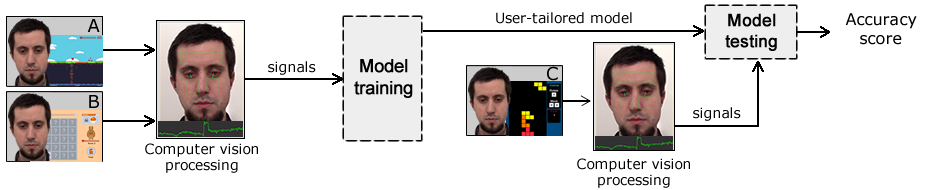
\includegraphics[width=\textwidth]{Content/figures/machine-learning-investigation.png}
    \caption{Iteration of a 3-fold \textit{Leave-One-Session-Out Cross-Validation} performed on the gaming session of a given subject with 3 games, i.e. A, B and C. Data of two calibration games, e.g. A and B, are used to train the machine learning model, while data of the third calibration game, e.g. C, is used to evaluate the model.}
    \label{fig:study5-training-evaluation}
\end{figure}

\textit{Leave-One-Session-Out Cross-Validation} (LOSOCV) is used to evaluate each trained user-tailored model, as illustrated in Figure \ref{fig:study5-training-evaluation}. In LOSOCV, data from one session instance is left out and a model is constructed on data from all other session instances. In the present study, a given subject $S_i$ played 3 calibration games, e.g. A, B and C, so data from one calibration game is left out and a model is trained on the data of the other two calibration games for that subject $S_i$. This is repeated for all three calibration games of that subject $S_i$. Consequentially the use of LOSOCV will produce 3 models per subject, resulting in 3 measurements of classificaiton accuracy per subject, denoted $L_j$, where $j \in \{1, 2, 3\}$ represent each evaluated model. The final classification accuracy for given subject $S_i$, named $A_i$, is calculated as the mean of $L_j$ values obtained from the iterations in the LOSOCV. In other words, each subject contributes a single classification accuracy value $A_i$, which is calculated based on the mean classification accuracy of his/her three models in the LOSOCV iterations.

In the training process of each model, which is performed 3 times per user, the hyper-parameters of each neural network, e.g. number of neurons, is optimized using random search \parencite{bergstra2012random}. A 10-fold cross validation method repeated 3 times is applied, so the dataset is split into 10-subsets and each of those subset is held out while the model is trained on all others. The process is repeated 3 times and the final metric for the model is the mean from the number of repeats. Area under the ROC curve (AUC) is used as a metric to select the best model.

According to previous analysis, subjects perceived the games as being boring at the beginning and stressful at the end. As a consequence, it is assumed that subject's emotional state in $H_0$ and $H_1$ is boredom and stress, respectively. Based on that assumption, training and evaluation data obtained from video segments in $H_0$ and $H_1$ were labeld as boredom and stress, respectively.

%, which finds models as good or beter then ones configured by a pure grid search

%Describe how the model was trained, which includes how the calibration games were grouped, e.g. two for training, one for testing. Explain that neural networks were used because they are widely mentioned in the literature.

%%%%%%%%%%%%%%%%%%%%%%%%%%%%%%%%%%%%%%%%%%%%%%%%%%%%%%%%%%%%%%%%%%%%%%%%
\subsubsection{Analysis}
\label{sec:experiment1-study5-analysis}
%%%%%%%%%%%%%%%%%%%%%%%%%%%%%%%%%%%%%%%%%%%%%%%%%%%%%%%%%%%%%%%%%%%%%%%%%

In order to test the effectiveness of the neural network in classifying samples as either boredom or stress, all trained neural networks were evaluated in conjunction. As described in the previous section, each subject's model was evaluated using LOSOCV, which produced a classification accuracy $A_i$ for any given subject $S_i$. The minimum, maximum and mean value of $A_i$ was calculated as a metric for accuracy. In order to better contextualize the classification results, the same process was also applied to other three metrics obtained during the LOSOCV evaluation: Precision, Recall and F1 score\footnote{F1 score should not be confused with $F_1$, the mouth outer facial feature used in the model.}. Precision accounts for the correctly predicted positive observations over the total of predicted positive observations, e.g. from all samples classified as stress, how many of those were indeed labeled as stress. Recall accounts for the correctly predicted positive observations over all available observations in a class, e.g. from all available samples labeled as boredom (or stress), how many were actually classified as such. Finally F1 score is the weighted average of Precision and Recall.

Aiming to better understand the contribution of each feature for the classification process, the training/evaluation process mentioned early was also performed using different feature sets. Each of those different feature sets was evaluated in an independent test, denoted $T_i$. Table \ref{table:study5-different-feature-sets} shows tests $T_i$ and the corresponding feature sets used in the process.

\begin{table*}
    \centering
    \caption{Tests and their respective feature sets}
    \label{table:study5-different-feature-sets}
    \begin{tabular}[l]{@{}cclp{4.0cm}}
        \toprule%
            \textbf{$T_i$} & \textbf{Name} & \textbf{Feature set} & \textbf{Note} \\
        \midrule%
            1 & \texttt{MULTI\_R} & $F_1^\mu$, $F_2^\mu$, $F_3^\sigma$, $F_4^\sigma$, $F_5^\mu$, $F_6^\sigma$, $F_8$ & Facial analysis, rPPG-estimated HR.\\ % 5278d175-71e752ce: HR_poh2011, mean_face_activity_mouth_corner, mean_face_activity_mouth_outer, mean_face_area, std_face_activity_eyebrow, std_face_eye_area, std_face_motion_instability
            2 & \texttt{MULTI\_G} & $F_1^\mu$, $F_2^\mu$, $F_3^\sigma$, $F_4^\sigma$, $F_5^\mu$, $F_6^\sigma$, $F_9^\mu$ & Facial analysis, HR from physical sensor.\\ % 5278d175-9fa716ee: mean_HR_ground, mean_face_activity_mouth_corner, mean_face_activity_mouth_outer, mean_face_area, std_face_activity_eyebrow, std_face_eye_area, std_face_motion_instability
            3 & \texttt{FACE} & $F_1^\mu$, $F_2^\mu$, $F_3^\sigma$, $F_4^\sigma$, $F_5^\mu$, $F_6^\sigma$ & Facial analysis only. \\ % 5278d175-826512b2: mean_face_activity_mouth_corner, mean_face_activity_mouth_outer, mean_face_area, std_face_activity_eyebrow, std_face_eye_area, std_face_motion_instability
            4 & \texttt{HR\_R} & $F_8$ & rPPG-estimated HR only.\\ % 5278d175-97a38001: HR_poh2011
            5 & \texttt{HR\_G} & $F_9^\mu$ & HR from physical sensor only. \\ % 5278d175-ad2580a5: mean_HR_ground
        \bottomrule%
    \end{tabular}
\end{table*}

Tests \texttt{MULTI\_R} and \texttt{MULTI\_G} use multifactorial set of features for their neural network, where facial and HR information are used in combination. The difference between \texttt{MULTI\_R} and \texttt{MULTI\_G} is that the former uses rPPG estimated HR, while the latter uses HR obtained from the physical sensor. Test \texttt{FACE} uses a set of features based solely on facial information. Finally tests \texttt{HR\_R} and \texttt{HR\_G} use only HR information as a feature. Similarly to \texttt{MULTI\_R} and \texttt{MULTI\_G}, tests \texttt{HR\_R} and \texttt{HR\_G} use HR readings from rPPG estimatations and from a physical sensor, respectively.

Subjects perceived the games as boring and stressful, so such difference should make a trained neural network capable of properly classifying evaluation samples as either boredom or stress. Additionally the use of a multifactorial approach, where facial analysis and HR information are used in combination instead of either one alone, is expected to produce better classification results \parencite{zacharatos2014automatic}. Based on those expectations, the following hypotheses are stated:

\begin{itemize}
  \item $u_1$: a user-tailored neural network trained on data samples from two calibration games of a given subject $S_i$ is able to classify samples from a third calibration game of that same subject $S_i$ with an accuracy greater than chance-level rate (random guessing);
  \item $u_2$: a user-tailored neural network using a multifactorial feature set, i.e. facial and HR features, performs with greater accuracy than a user-tailored neural network using facial features only;
  \item $u_3$: a user-tailored neural network using a multifactorial feature set, i.e. facial and HR features, performs with greater accuracy than a user-tailored neural network using HR features only.
\end{itemize}

Hypothesis $u_1$ was tested by checking if the mean value of the classification accuracy, i.e. calculated from all $A_i$ values, is greater than 0.5. In such case it is assumed that an accuracy rate of 0.5 (50\%) is the theoretical probabilistic chance level achieved by totally random classification performed by a classifier evaluated on an infinite number of data samples. Hypotheses $u_2$ and $u_3$ were tested by performing a Wilcoxon Signed Ranks test on all $J_i$ values of the two competing tests $T_i$. As previously mentioned, the use of LOSOCV produces 57 accuracy measuraments $J_i$ per test $T_i$.

%%%%%%%%%%%%%%%%%%%%%%%%%%%%%%%%%%%%%%%%%%%%%%%%%%%%%%%%%%%%%%%%%%%%%%%%%
\subsection{Results}
%%%%%%%%%%%%%%%%%%%%%%%%%%%%%%%%%%%%%%%%%%%%%%%%%%%%%%%%%%%%%%%%%%%%%%%%%

Table \ref{table:study5-result-metrics-mean} presents the mean values of the resulting classification metrics for accuracy, precision, recall and F1 score, calculated and analyzed according to the procedures described in Section \ref{sec:experiment1-study5-method}. Regarding the accuracy metric, the highest mean value achieved was 62.3\% in test \texttt{MULTI\_G}, whose model used a combination of facial and HR features. The HR feature in that case was calculated from the physical sensor, not remotely estimated. The second and third highest accuracy rates were 60.8\% in test \texttt{HR\_G} (HR from physical sensor only) and 60.4\% in test \texttt{MULTI\_R} (facial and remotely-estimared HR features), respectively. The highest values achieved for precision, recall and F1 score were 65.6\%, 62.4\%, and 58.1\%, respectively, all in test \texttt{HR\_G}.

\begin{table*}
    \centering
    \caption{Mean values of resulting classification metrics}
    \label{table:study5-result-metrics-mean}
    \begin{tabular}[l]{@{}ccccc}
        \toprule%
            \textbf{Test} & \textbf{Accuracy} & \textbf{Precision} & \textbf{Recall} & \textbf{F1}\\
        \midrule%
            \texttt{MULTI\_R} & 0.604 & 0.612 & 0.599 & 0.521 \\ % 5278d175-71e752ce
            \texttt{MULTI\_G} & \textbf{0.623} & 0.583 & 0.607 & 0.514 \\ % 5278d175-9fa716ee
            \texttt{FACE} & 0.594 & 0.601 & 0.585 & 0.507 \\ % 5278d175-826512b2
            \texttt{HR\_R} & 0.547 & 0.541 & 0.545 & 0.497 \\ % 5278d175-97a38001
            \texttt{HR\_G} & 0.608 & \textbf{0.656} & \textbf{0.624} & \textbf{0.581} \\ % 5278d175-ad2580a5
        \bottomrule%
    \end{tabular}
\end{table*}

Table \ref{table:study5-result-metrics-minmax} presents a discrimination of the minumum and maximum mean values for the resulting classification metrics. At least one subject in test \texttt{MULTI\_G} has been classified with a mean accuracy of 98\%, the highest value for that metric in all tests. The worst mean accuracy value was 19\% for at least one subject in test \texttt{MULTI\_R}. Regarding precision, the highest mean value was 97\% in test \texttt{MULTI\_G}. In all tests but \texttt{HR\_G}, at least one subject has been classified with zero precision (all samples were classified wrongly). Regarding precision, the highest and lowest mean values were 98\% and 12\% in tests \texttt{MULTI\_G} and \texttt{FACE}, respectively. Finally regarding F1 score, the highest mean value was 98\% for at least one subject in test \texttt{MULTI\_G}. All tests presented zero as the lowest F1 score.

\begin{table}[!htbp]
  \centering
  \caption{Minimum and maximum mean values of resulting classification metrics}
  \label{table:study5-result-metrics-minmax}
  \begin{tabular}{ccccccccc}
    \toprule%
      \textbf{Test} & \multicolumn{2}{c}{\textbf{Accuracy}} & \multicolumn{2}{c}{\textbf{Precision}} & \multicolumn{2}{c}{\textbf{Recall}} & \multicolumn{2}{c}{\textbf{F1}} \\
      {} & min & max & min & max & min & max & min & max \\
    \midrule%
      \texttt{MULTI\_R}  & 0.19 & 0.91 & 0.00 & 0.95 & 0.19 & 0.87 & 0.00 & 0.91 \\ % 5278d175-71e752ce
      \texttt{MULTI\_G}  & 0.25 & \textbf{0.98} & 0.00 & \textbf{0.97} & 0.13 & \textbf{0.98} & 0.00 & \textbf{0.98} \\ % 5278d175-9fa716ee
      \texttt{FACE}  & 0.26 & 0.90 & 0.00 & 0.95 & 0.12 & 0.90 & 0.00 & 0.89 \\ % 5278d175-826512b2
      \texttt{HR\_R}  & 0.36 & 0.72 & 0.00 & 0.79 & 0.18 & 0.77 & 0.00 & 0.67 \\ % 5278d175-97a38001
      \texttt{HR\_G}  & 0.38 & 0.82 & 0.26 & 0.85 & 0.23 & 0.87 & 0.00 & 0.81 \\ % 5278d175-ad2580a5
    \bottomrule%
  \end{tabular}
\end{table}

% data_multi_r and data_hr_r: p = 0.04488, Zstat = -2.0058, effect = 0.2657
% data_multi_r and data_face: p = 0.26797, Zstat = -1.1077, effect = 0.1467

Finally there are indications that a multifactorial model, which uses a combination of facial and HR features, performs with greater accuracy than a model using either facial or HR features. A Wilcoxon Signed Ranks test indicates that the mean accuracy was greater for a multifactorial model using facial and remotely estimated HR features, i.e. \texttt{MULTI\_R}, than for a model using only remotely estimated HR, i.e. \texttt{HR\_R}, $Z=-2.00$, $p=0.044$, $r=0.26$. However there are no indications that the mean accuracy of such multifactorial model, i.e. \texttt{MULTI\_R}, is statistically significantly greater than the mean accuracy of a model using only facial features, i.e. \texttt{FACE}, $Z=-1.10$, $p=0.267$, $r=0.14$.

%%%%%%%%%%%%%%%%%%%%%%%%%%%%%%%%%%%%%%%%%%%%%%%%%%%%%%%%%%%%%%%%%%%%%%%%%
\subsection{Discussion}
%%%%%%%%%%%%%%%%%%%%%%%%%%%%%%%%%%%%%%%%%%%%%%%%%%%%%%%%%%%%%%%%%%%%%%%%%

% data_multi_g and data_face: p = 0.03343, Zstat = -2.1269, effect = 0.2817
% data_multi_g and data_hr_g: p = 0.27802, Zstat = -1.0848, effect = 0.1437

% data_multi_g and data_multi_r: p = 0.07836, Zstat = -1.7603, effect = 0.2332

Results indicate that the use of a user-tailored model to remotely estimate the emotional state of players from videos of gaming sessions is feasible. Previously mentioned hypothesis $u_1$ states that a user-tailored neural network trained on data samples from two calibration games of a given subject $S_i$ is able to classify samples from a third calibration game of that same subject $S_i$ with an accuracy greater than chance-level rate (random guessing). Such model was tested in two configurations: \texttt{MULTI\_R} and \texttt{MULTI\_G}. Model \texttt{MULTI\_R}, which uses a multifactorial feature set composed of facial and remotely estimated HR information, presented a mean classification accuracy of 60.4\%. Such reported accuracy is greater than 50\%, the theoretical probabilistic chance level, which confirms hypothesis $u_1$. Model \texttt{MULTI\_G}, which also uses a multifactorial feature set but differs in the acquisition of HR data, i.e. physical sensor instead of remote estimation, presented a mean classification accuracy of 62.3\%. Such reported accuracy is also greater than the theoretical probabilistic chance level. The slightly greater classification accuracy of model \texttt{MULTI\_G} compared to \texttt{MULTI\_R} suggests that more precise rPPG estimations of the HR could improve the overall classification accuracy of model \texttt{MULTI\_R}. A Wilcoxon Signed Ranks test, however, has no statistically significant indication that the accuracy was greater for \texttt{MULTI\_G} than for \texttt{MULTI\_R}, $Z=-1.76$, $p=0.078$, $r=0.23$. Despite not being statistically significant, values $p=0.078$ and $r=0.23$ (small effect according to Cohen's classification of effect size) suggest a trend towards that reasoning.

Hypothesis $u_2$ states that a user-tailored neural network using a multifactorial feature set performs with greater accuracy than a user-tailored neural network using facial features only. The Wilcoxon Signed Ranks test mentioned in the previous section presented no statistically significant indications that the classification accuracy of \texttt{MULTI\_R} is greater than \texttt{FACE}. It is possible to speculate that a set of facial features, e.g. eyebrow and mouth analysis, has a greater potential to differentiate emotional states in a classifier. Particularly it might perform better than a classifier based on rPPG-estimated HR alone.

Regarding hypothesis $u_3$, which states that a user-tailored neural network using a multifactorial feature set performs with greater accuracy than a user-tailored neural network using HR features only. The Wilcoxon Signed Ranks test mentioned in the previous section presents statistically significant indications that the classification accuracy of \texttt{MULTI\_R} is greater than \texttt{HR\_R}. It supports the claim of hypothesis $u_3$, confirming that a multifactorial model performs better than one based solely on remotely estimated HR data. The lower classification potential of remotely estimated HR, however, could be attributed to errors in the rPPG estimation process caused by noise, e.g. natural movement of subjects (see Section \ref{sec:experiment1-study3}, on page \pageref{sec:experiment1-study3}, for more information). As a consequence, a more precise HR estimation used in a multifactorial model allegedly contributes to produce a better classifier. A Wilcoxon Signed Ranks test confirms with statistical significance that the classification accuracy of \texttt{MULTI\_G}, i.e. facial and HR from sensor, is greater than the accuracy of \texttt{FACE}, i.e. facial information only, $Z=-2.12$, $p=0.033$, $r=0.28$. It supports the previously mentioned idea that a precise HR estimation (from a physical sensor in the case of \texttt{MULTI\_G}) combined with facial information is a better classifier than one using facial information alone, i.e. model \texttt{FACE}. Finally a Wilcoxon Signed Ranks test does not indicate that the accuracy of \texttt{MULTI\_G} is greater than \texttt{HR\_G}, $Z=-1.08$, $p=0.278$, $r=0.14$. Consequentially it seems that precise estimations of HR is important, but HR or facial information used separately are likely to be less important for classification then a joint, multifactorial use of them in the emotion classification process.

Finally it is important to highlight the possible limitations of using the theoretical probabilistic chance level rate of 50\% for the evaluation of the model's accuracy. As previously mentioned, an accuracy baseline of 50\% assumes a totally random classification evaluated on an infinite number of data samples. One could argue that such scenario is unrealistic. In that case, the true evaluation of a model must consider statistical significance levels taking into account the sample size used in the process. \textcite{combrisson2015exceeding} present a work in the field of brain signal classification that uses analytical and empirical solutions, i.e. binomial formula and permutation tests, to show the influence of small numbers of data samples in the theoretical probabilistic chance level. According to the authors, a minimal correct classification rate of 62.5\% is required to assert statistical significance, i.e. $p < 0.05$, during the classification of two classes with a sample size of 40. In the present study, each subject was evaluated with 38 samples on average\footnote{This number refers to the amount of samples used for the evaluation of a model, not its training. During the training phase of each model, more than 38 samples were used per subject.}. As presented in the results of this study, the mean accuracy rate of models \texttt{MULTI\_R} and \texttt{MULTI\_G} are 60.4\% and 62.3\%, respectively. Following the analysis of \textcite{combrisson2015exceeding}, the mean accuracy rate of those multifactorial models would not be enough to assert statistical significance of the results. Nevertheless both models presented a mean accuracy that trends towards the minimal 62.5\%. Additionally the previously mentioned Wilcoxon Signed Ranks test does not indicate that the accuracy was greater for \texttt{MULTI\_G} than for \texttt{MULTI\_R}, so their performance could be the same. It is also important to stress the use of Leave One Session Out Cross Validation in the evaluation of each subject. It uses a completely independent and different game as source of sampling for the evaluation of each model, which strengthens the evaluation process. The reduced number of subjects in the study, i.e. 19, and the reduced number of samples used in the evaluation of each models, i.e. 38 on average, are in fact limiting factors. Reported results, however, provide insights regarding the feasibility of a multifactorial remote approach for emotion classification. The accuracy of the models presented in this study are not statistically confirmed without the assumption of baseline produced by a random classifier evaluated on an infinite number of data samples. However there is in fact a trend indicating that the use of a user-tailored model to remotely estimate emotional states of players is worth of further investigation.

% From: https://www.sciencedirect.com/science/article/pii/S1053811916000604#bb0235
% Recently, Combrisson and Jerbi (2015) compared the various statistical tests used to evaluate decoding performance and showed that the theoretical chance level was less stringent for small numbers of data samples, as found in neuroimaging studies, causing a bias towards statistical significance. The permutation test, by contrast, is not open to this criticism because it is a data-driven method and does not make assumptions about the statistical properties of the dataset. Therefore, the significance test we used may have been more stringent than the one used by those obtaining positive decoding findings in FFA.

%%%%%%%%%%%%%%%%%%%%%%%%%%%%%%%%%%%%%%%%%%%%%%%%%%%%%%%%%%%%%%%%%%%%%%%%%
\subsection{Conclusions}
%%%%%%%%%%%%%%%%%%%%%%%%%%%%%%%%%%%%%%%%%%%%%%%%%%%%%%%%%%%%%%%%%%%%%%%%%

This study presented a systematic evaluation of the feasibility of using a user-tailored neural network trained on data samples from two calibration games of a given subject to classify emotional states from a third calibration game of that same subject. Further investigation is required, however results suggest that a user-tailored neural network, based on remotely acquired data from video recordings, is able to classify emotional states with an accuracy greater than chance-level rate (random guessing).

Regarding the efficiency of a multifactorial model, where facial and HR information are together instead of separately, there are no statistically significant indications that the classification accuracy of such a model is greater than a model using facial information alone. However a multifactorial model based on remotely acquired data performs better than one based solely on remotely estimated HR data.

Finally it seems that precise estimations of HR is important, but HR or facial information used separately are likely to be less important for classification than a combined use of them in a multifactorial emotion classification model based on remotely acquired data. The analysis performed in this study supports further investigation regarding a user-tailored model to remotely estimate emotional states of player.

